\documentclass[12pt, a4paper, openany, oneside]{book}
\usepackage[italian]{babel}
\usepackage[T1]{fontenc}
\usepackage[utf8]{inputenc}
\usepackage{amsmath} 
\usepackage{xcolor}
\usepackage{listings}
\usepackage{hyperref}
\usepackage[margin=1in]{geometry}
\usepackage{graphicx}
\usepackage{amssymb}
\graphicspath{{./img/}}
\definecolor{britishracinggreen}{rgb}{0.0, 0.26, 0.15}
\newcommand\tab[1][1cm]{\hspace*{#1}}
\begin{document}
\fontfamily{cmss}\selectfont
\author{\href{https://github.com/daverhapsody}{DaveRhapsody}}
\title{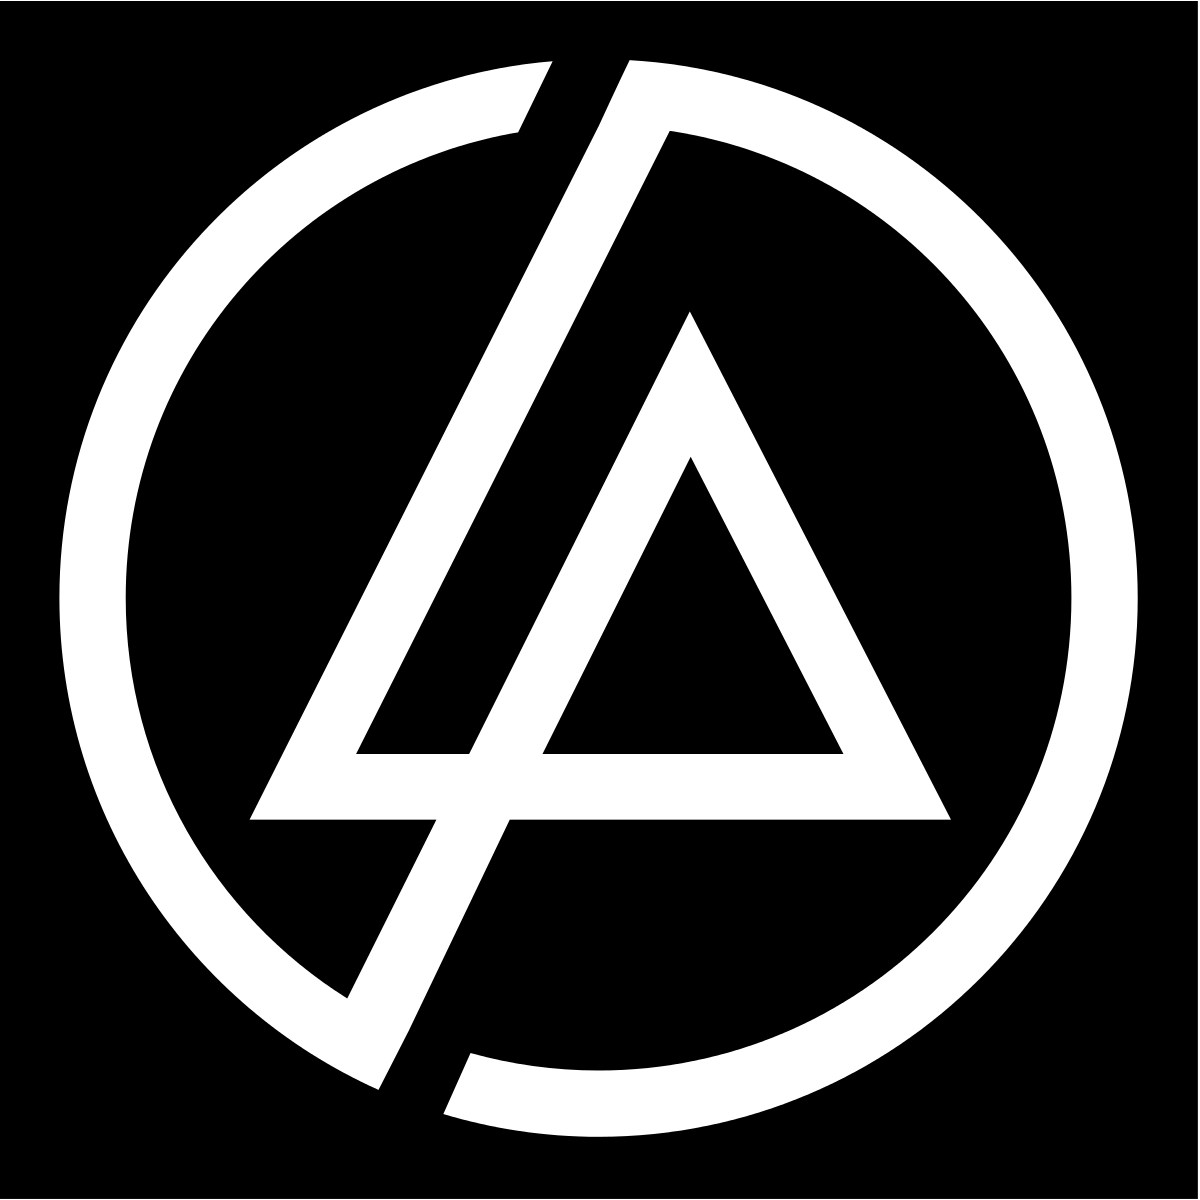
\includegraphics[width=0.10\textwidth]{logo}\\ 
Linguaggi di Programmazione}
\color{blue}
\date{30 Settembre 2019}
\color{black}
\maketitle
\tableofcontents
\chapter{Introduzione al corso}
\section{Programma del corso}
Il corso è volto ad insegnare dei paradigmi di programmazione dei seguenti tipi:
\subsection{Logica Matematica e Linguaggi logici (Prolog)}
Termini, fatti(predicati), regole, unificazione, procedura di risoluzione
\subsection{Linguaggi funzionali e Lisp (et al.)}
Atomi, liste, funzioni e ricorsione
\subsection{Linguaggi imperativi}
\label{sub:linguaggi_imperativi}
Memoria, stato, assegnamenti, puntatori
\\ 
{\color{black} \rule{\linewidth}{0.3mm} }
\\
Il concetto è che con questo corso si vanno a studiare paradigmi più evoluti,
usati tutt'ora e comunque aventi un ampio approccio logico, oltretutto LISP è 
usato nelle pagine web (Si userà moltissimo la ricorsione, A I U T O)
\section{Modalità d'esame}
\label{sec:modalità_d_esame}
\begin{itemize}
	\item il voto finale sarà una media pesata dei voti conseguiti nell'esame 
	relativo alla parte teorica e nell'esame del progetto 
	\begin{itemize}
		\item Occhio, il peso è a discrezione dei prof
	\end{itemize}
\end{itemize}
\subsection{Prove parziali}
\label{sub:prove_parziali}
Le prove d'esame sono costituite da uno scritto di 6-10 domande, e da un 
progetto da consegnare entro una data prefissata
\section{Appelli regolari}
\label{sec:appelli_regolari}
Gli appelli regolari sono composti da un progetto ed un esame scritto, che può
essere seguito da un esame orale a discrezione del docente basato sui temi 
trattati durante il corso
\\
\textbf{NON C'E' POSSIBILITA' DI RECUPERI}, infatti scritto, orale e progetto 
vanno sostenuti \color{red} \textbf{NELLO STESSO APPELLO} \color{black}
\\
Progetto e scritto sono corretti separatamente
\paragraph{NON CI SARANNO ECCEZIONI}
\label{par:non_ci_saranno_eccezioni}
Lo avete già letto nel passaggio precedente, ma lo ripeto lo stesso perchè 
deve essere chiaro che N O N  S I  F A N N O  E C C E Z I O N I.
%------------------------------------------------------------------------------
\chapter{Il paradigma}
\section{Cos'è?}
E' il metodo di soluzione ad un determinato problema, a seconda dei paradigmi si
hanno diversi tipi di linguaggi di programmazione
\subsection{Storicamente}
Il primo paradigma è l'imperativo, cioè il paradigma basato sui tre costrutti
di selezione, iterazione e sequenza. \\
Inoltre si mantiene il concetto di assegnamento di un valore ad una determinata variabile
\subsection{L'effetto collaterale}
Viene definito effetto collaterale quando, a seguito dell'esecuzione di un qualsiasi
codice, il contenuto di un'area di memoria viene cambiato; per intenderci, anche
solo l'istruzione "x += 1" genera un effetto collaterale, poichè nell'area di 
memoria di x viene cambiato il valore. \\
Perchè è importante tutto ciò, direte. Semplice: il paradigma puro funzionale si 
basa proprio sul fatto che un programma non generi mai, mai, \emph{M A I}, effetti 
collaterali.
Successivamente vedremo che in Prolog ci saranno parecchi problemi se provassimo
ad assegnare direttamente un valore ad una variabile
\section{Logica del primo ordine}
Prolog è costituito da una serie di clausole derivanti dalla logica del primo
ordine
\section{Linguaggi funzionali}
Questi si basano proprio sui concetti matematici di funzione, ad esempio si 
ragiona sui domini, sui codomini, sull'insiemistica, solite cose. La loro caratteristica
è che ogni funzione, dato sempre lo stesso input, restituisce sempre lo stesso
risultato. Cosa vuol dire questo? Che non dipende da variabili esterne (e da qui
l'importanza degli effetti collaterali, evitati nei linguaggi funzionali).
%------------------------------------------------------------------------------
\section{Paradigma imperativo}
Le caratteristiche essenziali dei linguaggi imperativi sono legate all'architettura 
di Von Neumann, costituita dai famosi due componenti 
\textbf{Memoria (componente passiva) e Processore (componente attiva)}
\\
In pratica la principale attività che ha la cpu è quella di eseguire calcoli
ed assegnare valori alle variabili, che sono delle celle di memoria.
\paragraph{Va considerato}
Il concetto di variabile è un'astrazione di una cella di memoria, per dire 
se giochi su assembly vai a toccare i veri e propri registri, mentre su C o 
Assembly si ragiona per nome di variabile, non vai di indirizzamento fisico
%------------------------------------------------------------------------------
\subsection{Il concetto di variabile}
In Prolog e LISP cambia completamente il concetto di variabile, ma per come 
saranno presentati vedremo che non c'entra niente. \\
In matematica abbiamo il concetto di variabile? Sì, quella che sta dentro una
funzione, in informatica è diciamo diverso, non è un'astrazione, ma lo vedremo
in seguito
\section{Modello di Von Neumann}
Per manipolare la memoria utilizzo la variabile, simbolo che indica la cella 
di memoria, nei linguaggi funzionali sarà possibile usare il concetto di 
variabile matematica. 
\\ \\
Alla fine il modello di Neumann è composto da I/O, Memoria e CPU con i suoi 
cicli di clock
\section{Stile prescrittivo}
Un programma scritto in un linguaggio imperativo prescrive le operazioni che
la CPU deve eseguire per modificare lo stato di un sistema \\ \\
Le istruzioni sono eseguite nell'ordine in cui queste appaiono, ad eccezione
delle strutture di controllo
\paragraph{Realizzati} sia attraverso interpretazione che compilazione, nati
più per manipolazione numerica che simbolica.
\\
\section{Concetto di programma}
Un programma è intendibile come un insieme di algoritmi e di strutture dati
ma la struttura di un programma consiste in
\begin{itemize}
	\item Una parte dichiarativa in cui son presenti le dichiarazioni di tutte
	le variabili del programma e del loro tipo
	\item Una parte che descrive l'algoritmo risolutivo utilizzato, mediante 
	istruzioni del linguaggio	
\end{itemize}
\section{Perchè utilizzare paradigmi diversi?}
Per esempio l'intelligenza artificiale si sviluppa su linguaggi di 
programmazione specifici, bisogna usare linguaggi che operino in un 
determinato modo, considerati tipo di Altissimo super mega galatticissifantastico 
livello infatti, utilizzabili pure da non programatori
\\ \\
Infatti son generati per manipolazione simbolica non numerica 
\section{Paradigma logico}
Concetto primitivo: Deduzione logica, avente una base di logica formale e un 
obbiettivo, che è intendibile come formalizzazione del ragionamento
\\ \\
\textbf{Programmare infatti significa} descrivere il problema con frasi 
(Formule logiche) del linguaggio, \\
Interrogare il sistema, che effettua deduzioni in base alla "conoscenza 
rappresentata" 
\paragraph{Ai lettori} Mi rendo conto che non si capisca un cazzo, voi 
immaginatevi come mi stia sentendo al momento io mentre prendo appunti.. 
Perdonatemi
\\ \\
Prolog è un insieme di formule ben formate, ragiona con il linguaggio logico, 
con una descrizione della realtà di interesse, di fatto è una dimostrazione in 
un linguaggio logico che costituisce un programma. Più semplicemente ho una  
frase da dare al mio interprete, Prolog icchè fa? Semplicemente la realizza  
sotto forma di dimostrazione. 
\\ 
\section{Esempio di un programma Prolog}
Ci sono fondamentalmente:
\begin{itemize}
	\item Asserzioni incondizionate (\color{red} fatti \color{black})
	A.
	\item Asserzioni condizionate (\color{red} regole \color{black})
	A :- B, C, D, ... , Z.
	\begin{itemize}
		\item A è la conclusione o conseguente (deve avere una sola clausola)
		\item B, C, D, \dots,Z sono le premesse o antecedenti 
	\end{itemize} 
	\item Un'\color{red}interrogazione \color{black} ha la forma: :- K, L, M, 
	\dots, P. \\
\end{itemize}
Ovviamente A, B, C, *TUTTE LE ALTRE*, sono semplicemente predicati
\\
MI RACCOMANDO MASSIMA ATTENZIONE ALLA SINTASSI, ogni clausola Prolog termina
con un punto. \\ \\
La ',' si legge come AND
\subsection{Esempio:}
Due individui sono colleghi se lavorano per la stessa ditta/azienda
\color{red} Regole \color{blue} Fatti \color{black} Interrogazione
\\ \\
\color{red}
collega(X, Y) :-  \\	
\tab lavora(X, Z), \\	
\tab lavora(Y, Z), \\	
\tab diverso(X, Y).
\\ \\
\color{blue}
lavora(ciro, ibm).  \\
lavora(ugo, ibm).  \\
lavora(olivia, samsung).  \\
lavora(ernesto, olivetti).  \\
lavora(enrica, samsung).
\\ \\
\color{black}
:- collega(X, Y). 
\\
{\color{black} \rule{\linewidth}{0.3mm} }
\\
Programmare Prolog non è come scrivere in un linguaggio di programmazione, non
si scrive un algoritmo, in questo caso abbiamo le famose clausole, (regole e 
fatti), 
\paragraph{ATTENZIONE} l'interrogazione non è una clausola, occhio a non confondersi
\subsection{Esempio dell'ordine di una lista}
\begin{itemize}
	\item \textbf{Ordine prescrittivo}: Controlla se la lista è vuota, e dà come 
	risultato la lista vuota stessa, altrimenti calcola una permutazione della 
	lista e controlla se è ordinata, dando come risultato $L_{1}$ altrimenti 
	fa una permutazione su L etc.
	\\
	Il programmatore deve specificare le istruzioni che generano la sequenza 
	di permutazioni della lista L
	\[
	\begin{cases}
	il ~ risultato ~ dell'ordinamento ~ di ~ una ~ lista ~ vuota ~ è ~ la ~ 
	lista ~ vuota \\
	Il ~ risultato ~ dell'ordinamento ~ di ~ una ~ lista ~ L ~ e ~ L_{1} 
	\end{cases}
	\]
	Quindi, lo stile prescrittivo presuppone che OGNI SINGOLO CASO venga considerato
	e programmato. non esiste il "ma è ovvio che debba fare questo", ogni singolo
	caso è tua responsabilità. Sì, tua, proprio tu che stai leggendo. Prolog si
	basa su questo tipo di ordine.
	\item \textbf{Stile Dichiarativo}: L'ambiente si fa carico di generare 
	possibili permutazioni della lista L, secondo deduzione matematica
\end{itemize}
\section{Paradigma funzionale}
\begin{itemize}
	\item 
	Si basa sul concetto di funzione matematica, ossia una associazione tra due 
	insiemi che relaziona ad ogni elemento di un insieme (dominio) un solo 
	elemento di un altro insieme (codominio)
	\item La definizione di una funzione specifica dominio, codominio, e regola
	di associazione 
	\\
	\item ESEMPIO: \\
	Incr: N $\to$ N \\
	Incr(x) - x + 1
	\item Dopo aver dato definizione, una funzione è aopplicabile ad un elemento del 
	dominio (argomento) per restituire l'elemento del codominio ad esso associato
	(valutazione)
	\item incr(3) $\to$ 4 
	L'unica operazione utilizzata nel funzionale è l'applicazione di funzioni  
	\item Il ruolo dell'esecutore di un linguaggio funzionale si esaurisce nel 
	calutare l'applicazione di una funzione (il programma) e produrre un valore 
	\item Nel paradigma funzionale puro il valore di una funzione è determinato 
	dagli argomenti che riceve al momento della sua applicazione e non dallo 
	stato del sistema rappresentato dall'insieme complessivo dei valori 
	associati a variabili(e/o locazioni di memoria) in quel momento 
	\item Oggettivamente si ha l'assenza di effetti collaterali \\ \\
\end{itemize}
\paragraph{Attenzione} % (fold)
\label{par:attenzione}
Il concetto di variabile che utilizziamo è quello di "costante" matematica, in 
cui i valori NON sono mutabili, non ho nessun asegnamento
\\ \\
L'essenza della programmazione funzionale consiste nel combinare funzioni 
mediante composizione e uso della ricorsione
% paragraph attenzione (end)
\subsection{Composizione di funzioni + ricorsione} 
La struttura di un programma consiste nella definizione di un insieme di 
funzioni ricorsive mutualmente
\\ \\
L'esecuzione del programma consiste nella VALUTAZIONE dell'APPLICAZIONE di una
funzione principale a una serie di argomenti
\section{LISP}
LISt Processing, \\ \\
Il progretto originale era di creare un linguaggio funzionale puro, infatti
nel corso degli anni sono stati sviluppati molti ambienti di sviluppo lisp
di cui terremo in considerazione Common Lisp e Scheme, oltre che emacs etc.
\subsection{Esempio di programma LISP}
Controlla un elemento se appartiene ad una lista \\ \\
\begin{lstlisting}[language=LISP]
(defun member (item list)) 
(cond ((null list)nil) 
((equal item(first list))T) 
(T(member item(rest list)))) 
(member 42(list 12 34 42))
\end{lstlisting}
Dopo una parentesi tonda ci va per forza una funzione, è fondamentale, defun 
definisce una funzione infatti, dopo c'è il nome di tale funzione. In LISP la 
tabulazione è ESSENZIALE, AUGURI A DISTINGUERE DOVE PORTI LA QUINTA PARENTESI DELLE 
DODICI CHE HAI SCRITTO PIANGENDO SUL CODICE ALLE 2 DI NOTTE.
\\
Gli elementi si separano con lo spazio NON con la virgola, mi raccomando.
\\
La terza riga è la più ostica e dice: è uguale T al primo elemento della lista?
E' molto incastrato ma si riesce a capire, associamo per esempio ad item = 2
(E' un esempio) e list = [1,2] \\
Noi ci arriviamo con la logica che c'è, ma in realtà cosa faremo? Ragioniamo 
per gradi
\begin{enumerate}
	\item null list? \color{magenta} false \color{black}
	\item è 2 = al primo elemento della lista? \color{magenta} False \color{black}
	\item è 2 = al secondo elemento della lista? \color{blue}True \color{black}
\end{enumerate}
Se LISP trova T è come se scrivessimo  \color{blue}\textbf{true}\color{black}
\section{Ambienti RunTime di linguaggi logici funzionali e non}
\begin{itemize}
	\item Richiami di nozioni di architettura e programmazione
	\item Per eseguire un programma di qualsiasi linguaggio il sistema operativo
	deve mettere a disposizione l'ambiente runtime che dia almeno due funzioni
	\begin{itemize}
		\item Mantenimento dello stato della computazione(pc, limiti di memoria)
		\item Gestione memoria disponibile (fisica e virtuale)
	\end{itemize}
	\item L'ambiente runtime può essere una vera e propria macchina virtuale tipo la JVM di java
	\item In particolare la gestione di memoria avviene usando due aree 
	concettualmente ben distinte con funzioni diverse
	\begin{itemize}
		\item Lo stack, ambiente dell'ambiente runtime che serve per la gestione 
		delle chiamate, a procedure metodi etc
		\item L'heap dell'ambiente runtime serve per gestire strutture dinamiche
		\begin{itemize}
			\item Alberi
			\item Liste etc
		\end{itemize}
	\end{itemize}
\end{itemize}
\subsection{Activation frame}
\begin{itemize}
	\item La valutazione di procedure avviene mediante la costruzione sullo
	stack di sistema di activation frames
	\item i parametri formali di una procedura vengono associati ai valori
	(si passa tutto per valore, non esistono effetti collaterali)
	\item E' un altro modo di chiamare i record di attivazione, via
	\item Il corpo della procedura viene valutato (ricorsivamente) tenendo 
	questi legami in maniera statica
\end{itemize}
cioè il concetto è che bisogna capire cosa accade con variabili che risultino 
libere in una sottoespressione
\section{Activation Frame di una funzione}
Contiene:
\begin{itemize}
	\item Return address
	\item Registri
	\item Static / Dynamic link (lo statico punta alle variabili globali)
	\item Argomenti
	\item Local definitions (RV)
\end{itemize}
Se si ha in mente come funziona oggettivamente lo stack (con i record di
attivazione) è la stessa cosa \\
All'esame si potrebbe chiedere cos'è l'activation frame e a icchè serve
\section{Heap e Garbage Collector}
L'heap è l'area di memoria destinata alla memorizzazione delle strutture per i
dati dinamiche, mentre invece il garbage collector ha il compito di accumulare
lo schifo che si accumula tra variabili non deallocate etc, e le dealloca 
appunto.
\chapter{Logica e ragionamento}
Partiamo con le cose semplici, bisogna passare da quello che è un linguaggio 
parlato a una stesura di condizioni \\
Prendiamo un triangolo, vogliamo dimostrare che se due triangoli hanno i due
lati uguali allora è isoscele \\
\[AB = BC \vdash \angle A \angle C\]
\begin{enumerate}
	\item AB = BC per ipotesi
	\item ABH = HBC per (Ipotesi 3)
	\item Il triangolo HBC è uguale al triangolo HBC ABH per (Ipotesi 2)
	\item A e C per (Ipotesi 1)
\end{enumerate}
\subsection{Regole di inferenza}
Esempio di una regola di inferenza:
\[
\frac{F_{1}, F_{2}, F_{3}, ..., F_{n}}{R}
\]
\begin{enumerate}
	\item Introduzione della congiunzione (L'AND)
	\item Modus Ponens
	\item Eliminazione della congiunzione
\end{enumerate}
Come lavora il \textbf{Modus Ponens}: \\
E' semplice manipolazione sintattica, osservando la formula che ci vien data
possiamo riscriverla scrivendo come base di conoscenza il conseguente, 
cioè in pratica prendo e sostituisco con il conseguente.
\\ \\
Per far si che le mie formule siano vere, se avessi un A or B può esser vera in 
ben tre casi diversi, non posso eliminare i due casi disgiunti, se voglio 
mantenere una solidità non posso, e quindi questa regola (disgiunzione) non 
esiste.
% consiglio di inserire un'immagine che mostri lo schema del modus ponens
\paragraph{Attenzione} in una dimostrazione non si può dare nulla per 
scontato, tutto ciò che noi diamo per assodato, un pc non lo dà, dobbiamo 
essere molto precisi nelle indicazioni, bisogna lavorare in un'ottica più 
precisa
\\ \\
cerchiamo ora di tradurre tutto in un linguaggio più formale
SE AB = BC E BH = BH e ABH = HBC allora il triangolo ABH è uguale a HBC 
ed abbiamo trasformato (1) in \\ \\
SE triangolo ABH è uguale al triangolo HBC ALLORA AB = BC e BH = BH e AH = HC,
E ABH = HBC E AHB = CHB E A = C
\\ \\
Da un punto di vista formale noi partiamo da un'ipotesi, noi vogliamo 
dimostrare che A = C.
\\ \\
La dimostrazione è un processo sintattico, non ragiono in termini di verità, 
perchè NON si sta parlando di interpretazione ma manipolazione delle formula
\\ \\
Ogni passo deve corrispondere ad una formula, e subito dopo le etichette
\paragraph{Differenza tra assiomi e ipotesi}
Gli assiomi sono conoscenza pregressa del dominio, mentre le ipotesi sono solo
supposizioni iniziali, uno si specifica, l'altro no
\section{Dimostrazione}
E' una sequenza di passi dove il finale è la formula da dimostrare e abbiamo
un insieme di passi intermedi che possono essere presi dalle conoscenze
pregresse, oppure applicando regole di inferenza ai passi PRECEDENTI, solo
precedenti mi raccomando.
\\ \\
Le regole di inferenza sono applicabili solo ai passi precedenti rispetto ad 
una formula
\section{Logica Proposizionale}
Nella logica proposizionale ci si occupa delle conclusioni che possiamo 
trarre da un insieme di proposizioni, abbiamo infatti un insieme P di 
proposizioni \\ \\
Si introduce il concetto di \textbf{interpretazione} di un insieme di 
proposizioni, infatti all'insieme P si associa una funzione di verità (True e 
False) \\ \\
Questa funzione associa un valore di verità ad ogni elemento di P, ad ogni 
proposizione. La valutazione è il ponte tra sintassi e semantica di un 
linguaggio \\
Posso derivare sintatticamente una formula, e se ho consistenza delle supposizione
avere comunque una formula.
\\ \\
Chiaramente posso legare tra loro le proposizioni con $\vee \wedge$ e $\neg$ 
Una formula ben formata è un insieme di espressioni sintatticamente corrette di
un linguaggio
\\
In prolog le formule atomiche le chiameremo letterali, che possono esser 
positivi e negativi, e qui si richiamano i concetti di fondamenti della tabella
di verità
\\ \\
Negli esercizi potremo usare 
\[\frac{F_{1}, F_{2}, ... , F_{K}}{R}\]
E' la forma generale di una regola, sopra hai l'insieme delle formule vere tra 
le formule ben formate e R è la formula generata da “inserire” in FBF. \\ \\
L'esempio di inferenza che si usa di solito è il Modus Ponens: 
\[\frac{p \to q, p}{q} \]
Se il conseguente appare come formula negata, si negherà anche la formula originaria
\subsubsection{Esempio:}
$\frac{p \vee \neg q}{vero} $ Terzo escluso \\ \\
$\frac{\neg \neg q}{q} $ eliminazione $\neg$ \\ \\
$\frac{p \wedge vero}{p} $ eliminazione $\vee$ \\ \\
$\frac{p \wedge \neg p}{q} $ contraddizione
\section{Principio di risoluzione}
E' una regola di inferenza generalizzata semplice e facile da utilizzare ed 
implementare, in pratica opera su formule ben formate trasformate in forme 
normali congiunte, ed ognuno dei congiunti vien detto \textbf{clausola}
\\ \\
L'osservazione fondamentale alla base del principio di risoluzione è un'estensione 
della nozione di rimozione dell'implicazione su base della contraddizione \\ \\
In pratica si usa per le dimostrazioni per assurdo.
\section{Unit Resolution}
E' un caso particolare di principio di soluzione; \\ \\
Da un lato ho una formula ben formata disgiuntiva e dall'altro ho un letterale 
(o asserito), e una di queste formule è costituita da un solo letterale, per 
questo si chiama unit, è sintassi, non ci sto capendo più un cazzo pure. 
io, non so davvero che dirvi.. \\ \\ 
\paragraph{Spiegazione fornita da } \href{https://github.com/JacopoDeAngelis}
{Jacopo De Angelis} \\ \\
Eccomi, arrivo da autore esterno a spiegare: prendiamo prima lo schemino semplice
semplice \\
$ P \leftarrow A \wedge B \wedge C \wedge D ...$ \\
Questo vuol dire che P è vera solo se tutte A, B, C e D sono vere. Ora, prendiamo 
nuovamente il codice prolog visto all'inizio: \\
\color{red}
collega(X, Y) :-  \\	
\tab lavora(X, Z), \\	
\tab lavora(Y, Z), \\	
\tab diverso(X, Y). \color{black}\\
Cosa cambia dal dire questo o la regola sopra? La corrispondenza è semplicemente: \\
\color{red}
\textbf{P} è collega(X, Y) :-  \\	
\tab \textbf{A} è lavora(X, Z), \\	
\tab \textbf{B} è lavora(Y, Z), \\	
\tab \textbf{C} è diverso(X, Y). \color{black}\\
Questo vuol dire che la nostra unit, P, è vera solo se sono vere le altre. Fine 
del mio intervento, la linea di nuovo a Dave.
\paragraph{Esempio:} 
\begin{itemize}
	\item <non piove>, <piove o c'è il sole>
	\item <c'è il sole>
\end{itemize}
La dimostrazione per assurdo di fatto funziona assumendo che la formula negata
sia vera, se combinandola con le proposizioni in fbf ottengo una contraddizione
, allora si pul concludere con la verità della proposizione.
%Da inizio capitolo a qua devo riguardare e completare con le cose mancanti
\subsection{Esempio di dimostrazione per assurdo}
Abbiamo una proposizione $\lambda$ e dobbiamo dimostrare che essa sia vera: \\
Per dimostrarlo occorre porre per ipotesi che $\neg \lambda$ sia vera e 
\color{red}SE \color{black} FBF U {$\neg \lambda$} genera una contraddizione,
\color{red}ALLORA \color{black} $\lambda$ è vera!
\section{Ricapitolando} 
Quello che noi definiamo come "Calcolo Logico" delle proposizioni va a toccare
\begin{itemize}
	\item Dal punto di vista della sintassi
	\begin{itemize}
		\item Un insieme di proposizioni che chiameremo \textbf{P}
		\item Un insieme di \textbf{FBF}, tale che \textbf{P}$ \subseteq$ \textbf{FBF}
		\item Un sottoinsieme di assiomi \textbf{A} $ \subseteq $ \textbf{FBF}
		\item Un insieme di regole di inferenza che ci permettono di 
		incrementare \textbf{FBF}
	\end{itemize}
	\item Dal punto di vista della Semantica
	\begin{itemize}
		\item Una funzione di verità che consente di distinguere \textbf{true} e
		\textbf{false} rispetto alle tavole di verità o funzioni di interpretazione
	\end{itemize}
\end{itemize}
\section{L'assioma}
Un assioma è una conoscenza che si da per assodata, qualcosa di sicuramente vero,
se vogliamo anche "scontato" 
\subsection{L'esempio dell'unicorno}
Se l'unicorno è mitico, allora è immortale, ma se non è mitico allora è mortale.
Se è mortale o immortale allora è cornuto. L'unicorno è magico se è cornuto. \\ \\
L'unicorno:
\begin{itemize}
	\item E' mitico?
	\item E' magico?
	\item E' cornuto?
\end{itemize}
\subsubsection{Procedimento}
\begin{enumerate}
	\item Esprimere il problema in forma di logica delle proposizioni
	\item Individuare i teoremi da dimostrare
	\item Dimostrare i teoremi
\end{enumerate}
Cioè concettualmente devo cercare di individuare i predicati, e porli in modo
più logico (Tipo mitico(x), magico(x) e cornuto(x)), MA MI RACCOMANDO ATTENZIONE.
\paragraph{NON CONFONDERE} I termini a disposizione, se qui hai mortale o "Immortale"
stai parlando di qualcosa che è Mortale $\vee \neg$ Mortale. \\
Ora andiamo a risolvere questo esercizio, e si comincia con il dare un nome
ai nostri predicati, che siccome sarebbero lunghi, saranno abbreviati in massimo
5 predicati
\begin{itemize}
	\item UM = Mitico
	\item UI = Immortale 
	\item UMag = Magico
	\item UC = Cornuto
\end{itemize}
Ritrascriviamo quindi la nostra frase iniziale: \\
UM $\to$ UI, \\
$\neg$UM $\to \neg$ UI, \\
$\neg$UI $\vee$ UI $\to$ UC \\
UC $\to$ UMag \\
Mentre per quanto riguarda le domande poste:
\begin{enumerate}
	\item S $\vdash$ UM ?
	\item S $\vdash$ UMag ?
	\item S $\vdash$ UC?
\end{enumerate}
Risolvendo l'esercizio otteniamo che
Ora, il metodo per risolvere le $\vdash$ potrebbe essere tramite negazione della
nostra ipotesi. In che senso? Proviamo con il caso S $\vdash$ UC \\ \\
\begin{itemize}
	\item P1: $\neg$ UI $\vee$ UI $\to$ UC (Da S)
	\item P2: $\neg$ UI $\vee$ UI (Che era stato dimostrato in un passaggio 
	precedente con la dimostrazione di A$\to$(B$\to$C))
	\item P3: UC (Da P1, P2 e modus ponens)
\end{itemize} 
% Proviamo ora a verificare per esempio se l'unicorno è magico. Riscriviamoci
% l'insieme $S = \{UM \implies UI, \neg UM \implies \neg UI, \neg UI \vee UI
%  \implies UC, UC \implies Umag\}$
Il compitino avrà un esercizio di questo livello di difficoltà che consisterà in
una dimostrazione, che ovviamente va per assurdo.
\subsection{Tautologie e modelli}
Una fbf che si verifica in ogni caso, è detta \textbf{Tautologia} (Fondamenti
docet)\\
Una particolare \textbf{Interpretazione} V che rende vere tutte le formule in
\textbf{S} viene detta \textbf{modello} di S
\section{La logica del primo ordine}
Se la logica proposizionale si dimostra utile, avente caratteristiche di 
computazione che da questo punto di vista sono chiare, c'è da dire che la 
semantica è chiara allo stesso modo, però purtroppo non ci permette di 
fare asserzioni in merito ad insieme di elementi in maniera concisa.
\paragraph{Ai lettori} Cioè io sto capendo logica adesso e non l'ho capita a 
Fondamenti.. Meditiamo ragazzuoli, meditiamo. \\
Sono Jacopo, vi parlo dal terzo anno. Fondamenti si capisce SOLO tramite gli 
altri corsi. \\ \\
\\
{\color{black} \rule{\linewidth}{0.2mm} }
\\
Con la \textbf{Logica del primo Ordine} introduciamo modi diversi di esprimere
le proposizioni, prendiamo per esempio Socrate (Ricordate Palmonari? Ecco)\\
\begin{itemize}
	\item Tutti gli uomini sono mortali
	\item Socrate è un uomo
	\item dalle precedenti ipotesi si deduce che Socrate è mortale
\end{itemize}
C'è un problemino di fondo, non si può esprimere in alcun modo qualcosa del tipo
"Tutti gli uomini sono mortali" \\ \\
Un linguaggio logico del primo ordine è costituito da \textbf{termini} che in 
pratica si costruiscono con 	
\begin{itemize}
	\item V: insieme di simboli di variabili
	\item C: insieme di simboli di costante
	\item R: insieme di simboli di relazione o predicati (di qualsiasi arietà)
	\item F: insieme di simboli di funzione (di qualsiasi arietà)
\end{itemize}
\paragraph{Ah, giusto} L'arietà sarebbe il numero di argomenti di una relazione o
predicato. (Chiaramente anche funzioni, in quanto caso particolare di relazione)
\\ \\
Inoltre si hanno i connettivi logici, ovvero $\forall$ (Per ogni) e $\exists$ 
(Esiste). \\ \\
In Prolog ci sarà un uso implicito dei quantificatori, è implicita la 
congiunzione, l'universale non è specificato ma è sottointeso, tutte le formule 
valgono assumendosi la quantificazione universale. 
\paragraph{Una sola causa} E' quantificata in modo esistenziale, la query. Se 
Però questa è una cosa che si gestisce l'interprete, noi non ci si fa problemi 
da questo punto di vista
\\ \\
Attenzione, in prolog non bisogna usare in modo intercambiabile simboli di 
predicato con quelli di funzione, perchè supponiamo la funzione "successore di 
un numero". La funzione successore dato un valore numerico $\lambda$, successore
mi darà $\lambda$ + 1.
\\ 
In questo caso ha simbolo di funzione, il predicato ti dà o vero o falso, pochi 
cazzi.
\\ \\
Se ho Successore(a, $\lambda$), questo mi dà true o false, è $\lambda$ successore
di a? Se sì mi dà true o altrimenti mi dà false. Questa è la differenza, oltre al
fatto che un predicato ragiona sul singolo argomento.
\\ \\
\paragraph{Postilla simpatica: }Quello che chiamo Modus Ponens, non è altro che 
un modo più simpatico di chiamare l'eliminazione dell'implicazione, che è quello
che facevamo a fondamenti, ma chiamiamolo modus ponens, perchè sì. 
\\ \\
Con la logica di primo ordine si ragiona diversamente, infatti il linguaggio
è costruito ricorsivamente, ed i termini minimi sono detti \textbf{PREDICATI}
\subsection{Le Formule Ben Formate nella logica del primo ordine}
Qui si fa menzione della definizione \textbf{Ricorsiva} di Formula Ben Formata
cioè:
\[FBF = \{t_{j}, r_{t_{1}, ... ,t_{k}}\}\]
Dove $t_{j}$ è un termine elemento di C, di V, oppure un'applicazione di una
funzione f($t_{1}, ... ,t_{s}$)\\ mentre
\[r(t_{1}, ... ,t_{k})\]
Che sarebbe un termine costituito da un predicato (dove le t derivano dai termini
appartenenti alle FBF) \\ \\
Contiamo che diversi elementi di FBF connessi dai connettivi $\forall , \exists
\neg, \to$ appartengono ad FBF
\paragraph{Si denota} t($t_{1}, ... ,t_{s}$) tale combinazione di termini \\
\\
{\color{black} \rule{\linewidth}{0.2mm} }
\\
Grazie alle definizioni precedenti possiamo andare a risolvere l'esempio di 
Socrate. \\
Iniziamo dalle cose semplici, definiamo chi sono le costanti (insieme C)$\to$ \\
Socrate è una costante, pertanto apparterrà all'insieme C: C = \{Socrate\}, e poi
possiamo definire quello che sono i predicati, che sono in questo caso uomo e 
mortale. \\ \\
I predicati appartengono all'insieme R; R = \{ uomo. mortale\} \\ \\
Benissimo, proviamo ora a realizzare la frase "Tutti gli uomini sono mortali": \\
Se tutti gli uomini son mortali, significa che per ogni elemento x tale che esso
sia un uomo, si implica che x sia mortale. 
\paragraph{Osservazione} Quando dico "Sia un uomo" e "Sia mortale", intendo che
la funzione uomo(x) e mortale(x) siano tendenzialmente delle booleane \\ \\
Infatti ritrascrivendolo vien fuori: $\forall$ x, (uomo(x)$\to$mortale(x)), 
tenendo conto che Socrate è un uomo, pertanto si dirà uomo(Socrate), che se
pensate al booleano, sì, darà \color{blue} \textbf{ true} \color{black}.
\subsection{Calcoli logici}
Per ottenere il risultato è necessario che si utilizzino delle regole di
calcolo %%(Soprattutto quelle legate al $\forall$ ed $\exists$ 
\subsubsection{Regola di eliminazione del quantificatore universale}
Il discorso è: Come si risolve il $\forall$?
\[\frac{\forall x, T(..., x, ...), c\in C}{T(..., c, ...)} \]
Si ok, ma come lo realizziamo?  \\ 
Con questa super mega iper formula possiamo finalmente derivare la nostra
conclusione a partire dalle asserzioni iniziali. 
\begin{enumerate}
	\item uomo(Socrate)
	\item $\forall$x, uomo(x) $\to$ mortale(x)
	\item mortale(Socrate)
\end{enumerate}
Andiamo a scrivercela sostituendo alla formula $\to$
\[\frac{(\forall x, uomo(x) \to mortale(x)), Socrate\in C}{uomo(Socrate)\to 
mortale(Socrate)}\]
Ora andiamo a togliere il quantificatore universale ($\forall$ detto in modo figo)
\[ \frac{uomo(Socrate), uomo(Socrate) \to mortale(Socrate)}{mortale(Socrate)}\]
Cosa notiamo? Il "denominatore" della prima formula è diventato il "numeratore"
della seconda, infatti vedete come abbiamo uomo(Socrate) $\to$ mortale(Socrate)?
\\ \\
A questo punto bisogna togliere anche l'implicazione, o meglio risolverla. 
Riflettendoci $A \to B$ a cosa è uguale? $\neg A \wedge \neg B$, in questo
modo abbiamo risolto l'implicazione.
\section{Altre regole in Logica del Primo Ordine}
Abbiamo risolto il $\forall$, ok, ma l'$\exists$?
Introduciamo quindi il quantificatore esistenziale:
\[
\frac{T(..., c, ...), c\in C}{\exists x, T(..., x, ...)} 
\]
Per completezza possiamo dedurre il fatto che 
\[
\begin{cases}
Se ~ \exists x, \neg T(..., x, ...) = \neg \forall x, T(..., x, ...) \\
Se ~ \forall x, \neg T(..., x, ...) = \neg \exists x, T(..., x, ...)
\end{cases} 
\]
Spiegato peggio, se dico che esiste un elemento, per cui non si verifica una 
proprietà, allora non per ogni elemento essa si verifica. \\ 
Spiegato ancora peggio, se uno solo non si verifica, allora significa che non 
tutte si verificano \\ \\
Nel secondo caso invece se dico che per ogni x una proprietà non si verifica,
allora non esiste alcun x per cui si verifica 
\paragraph{Precisazione} In effetti negare il $\forall$ si tradurrebbe in 
"non tutte le x", mentre è molto più semplice per l'$\exists$ in cui si dice
"non esiste", lo specifico perchè io mi ci confondevo spesso.
\chapter{Prolog}
\paragraph{Prima ancora di cominciare: } Siccome mi seccava scaricarmi tutto 
l'ambiente di sviluppo Swi-Prolog, vi lascio qui sotto il link per avere il 
compilatore direttamente online che OVVIAMENTE non è utilizzabile all'esame, 
però fa comodo, ve lo assicuro. \href{https://swish.swi-prolog.org/}
{Link al magico sito}
\\
{\color{black} \rule{\linewidth}{0.3mm} }
\\ 
Data questa confusissima introduzione giungiamo a trattare più nello specifico
il linguaggio Prolog. Quando parliamo di Prolog, infatti, smettiamo di ragionare
in modo \color{red} \textbf{imperativo} \color{black} per passare al paradigma 
di \color{red} \textbf{programmazione logica} \color{black}.
\paragraph{Premessa: }C'è (come lo è stato per Prog 1) da scaricarsi l'interprete
di Prolog, si consiglia SWI-Prolog, che si appoggia ad Emacs come editor di testo.
\\ \\
(Sia per la stesura di questi appunti che per gli esercizi io ho sempre usato
Sublime Text MA all'esame molto probabilmente dovremo usare quel che ci impongono
loro, pertanto, meglio abituarsi da subito ad Emacs.)
\section{Programmazione logica}
Se prolog utilizza il paradigma di \color{red} \textbf{programmazione logica} 
\color{black}, quest'ultima non è rappresentata solo da Prolog, ci sono ovviamente
altri linguaggi che lo fanno. Perchè scegliere Prolog?
\begin{itemize}
	\item Il formalismo è più semplice
	\item E' un linguaggio ad alto livello
	\item La semantica è comprensibile
\end{itemize}
Quello che è il nostro programma divente un \color{red} insieme di formule
\color{black} ed ha un enorme potere espressivo, mantenendo come chiave il fatto
che la computazione effettiva è costruzione di una dimostrazione di una affermazione
(Definita anche come goal, obbiettivo, meta).
\subsection{Logica Matematica}
\paragraph{Definizione Davis e Putnam: } Per logica matematica si intende la
dimostrazione automatica di teoremi, secondo Davis e Putnam la logica matematica
implica la dimostrazione dei teoremi
\paragraph{Definizione Kowalski: } Interpretazione procedurale di formule. 
Quindi in pratica qua si entra già più nel concetto di un linguaggio
di programmazione.
\section{Cos'è ProLog}
Nel titolo di questa sezione la L maiuscola non è a caso, perchè Pro-Log sarebbe
acronimo di \textbf{PRO}gramming \textbf{LOG}ic, ed è un linguaggio che si basa
su una restrizione della logica del primo ordine (FOL).
\subsection{Ambiti di applicazione}
Generalmente prolog è utilizzato come linguaggio per gestire i Database, 
tendenzialmente alcuni DBMS (Database Management System) sono programmati 
\subsection{Caratteristiche di Prolog}
\begin{itemize}
	\item Si basa su una restrizione della logica del primo ordine
	\item Ha uno stile dichiarativo
	\item E' usato per determinare quando una affermazione è vera e quali vincoli
	abbiano fatto da discriminante tipo i vincoli sui valori da dare alle 
	variabili che han generato la risposta
\end{itemize}
\section{Formule Ben Formate e Forma Normale a clausole}
Qualsiasi formula ben formata può essere riscritta in forma normale a clausole.
Esistono due forme normali a clausole:
\begin{enumerate}
	\item Forma congiunta: \\
	La formula è una congiunzione di disgiunzioni di predicati o negazioni di 
	predicati (letterali positivi e letterali negativi) \\ 
	\[\bigwedge \limits_{i} (\bigvee \limits_{j} L_{ij})\]
	\item Forma disgiunta: \\
	E' una disgiunzione di congiunzioni di predicati o negazioni di predicati
	(letterali positivi e letterali negativi)
	\[\bigvee \limits _{j} (\bigwedge \limits _{i} L_{ij})\]
\end{enumerate}
\subsection{Forma normale disgiuntiva}
La clausole che hanno al più un solo letterale positivo (sia con che senza 
letterali negativi) si chiamano clausole di \color{red} \textbf{Horn} \color{black}
\\ \\
Spiegato meglio, perchè così non è chiaro in effetti, in pratica prendete una 
clausola a caso: $A \wedge B \vee \neg C $, è una clausola di Horn perchè c'è
UN SOLO TERMINE (Letterale) che NON è \textbf{Negativo}. (O \textbf{Negato})
\\ \\
\paragraph{Precisazione: } Se abbiamo un solo letterale positivo, esso è clausola
di Horn pure non c'è nemmeno un letterale negativo,  ne basta uno solo positivo.
\\ \\
Però occhio:
Non tutte le formula ben formate si riescono a far diventare un insieme di 
clausole di Horn, che per la cronaca compongono i programmi Prolog o meglio, 
\color{blue} \textbf{I programmi prolog son collezioni di clausole di Horn} 
\color{black}
\\ \\
Le suddette clausole rappresentano (lo si analizzerà successivamente) fatti, 
regole o interrogazioni (query/goals).
\subsection{Linguaggio dichiarativo}
Uno dei punti di forza di Prolog è il fatto che sia un linguaggio dichiarativo,
quindi è pressochè esente dall'avere istruzioni, contiene solo fatti e regole,
che dal passaggio precedente sappiamo essere delle \color{blue} 
\textbf{clausole di Horn} \color{black}. 
\paragraph{Ricordiamo che: } Un fatto è una asserzione vera nel contesto che si 
descrive, tipo assioma, mentre la regola è qualcosa che serve per dedurre dei 
nuovi fatti \textbf{partendo} da quelli esistenti. \\ \\
Un programma scritto in Prolog ci dà informazioni su un sistema, e vien chiamato
\color{red} base di conoscenza \color{black} (Il programma eh, non il sistema.)
\\ \\
Inoltre, (\textit{già detto in precedenza ma va ripetuto perchè sicuramente anche io 
stesso quando andrò a studiare da qua mi sarò già dimenticato}) un programma 
Prolog \color{red} \textbf{non si esegue} \color{black}, ma si \textbf{interroga}.
\\ \\
Quali sono le possibili domande da fargli? Ad esempio:
\begin{itemize}
	\item Questa serie di fatti è vera? \\
	E la risposta sarà \color{britishracinggreen}Si \color{black} o \color{red}No, 
	\color{britishracinggreen}True \color{black} o \color{red}False, \color{britishracinggreen}1
	\color{black} o \color{red}0, \color{britishracinggreen}"Si broh" \color{black} o 
	\color{red}"No frate".
\end{itemize}
Più precisamente questo sì sarebbe un "Sì, ho dimostrato il mio teorema per 
assurdo", perchè appunto ricordiamo che qua si sta parlando comunque di 
dimostrazione di teoremi
\section{Sintassi Prolog}
\begin{itemize}
	\item Fatto/Asserzione: *nomefatto*. 
	\item Regole: c :- $b_{1}, ..., b_{n}$.
	\item Goal/Query: ?-$q_{1}, ..., q_{n}$.
	\paragraph{Inciso: }Queste vanno scritte nel terminale, non nel programma.
	Sono tipo richieste che noi facciamo in base al momento per intenderci. 
\end{itemize}
Quando l'interprete prolog si trova di fronte una query (o goal) esegue in 
sequenza la unit resolution andando in sequenza sulle sue clausole, dalla prima
all'ultima, e le valuta tutte perchè potrei avere parecchie differenti soluzioni, 
posso dimostrare più teoremi.
\\ \\
Ogni lettera avente un pedice tipo $p_{\lambda}$ o $q_{\kappa}$ sono tutti 
termini composti, notare che in molte implementazioni il prompt Prolog è anche 
un operatore che chiede al sistema di valutare il \color{blue} goal \color{black}
\\ \\
Ogni espressione Prolog diventa \textbf{TERMINE}, ne abbiamo diversi esempi:
\begin{itemize}
	\item Atomi: \\
	E' una semplice sequenza di caratteri che inizia con carattere \textbf{Minuscolo}
	e può avere il '\_', oppure è un numero, o qualcosa racchiusa tra apici (' ') 
	\item Variabili
	\item COmposizioni di altri termini (Da qui termine composto)
\end{itemize}
NB. Tutto ciò riguarda la sintassi, questo elenco è legato al "Come si scrive 
questa determinata cosa in Prolog" 
\paragraph{Precisazione}
Ogni istruzione finisce con il punto, avete presente quando la vostra fidanzata
capite che è innervosita con voi e alla fine delle frasi ci mette un '.' che vi
fa gelare il sangue? Ecco, se qui non mettete il punto dopo ogni istruzione, 
vedrete come vi gireranno i *\textit{Censura}* ;))))\\ 
\paragraph{Ecco un esempio di comandi validi (\LaTeX ~ le metterà nella prossima 
pagina)}
\begin{center}
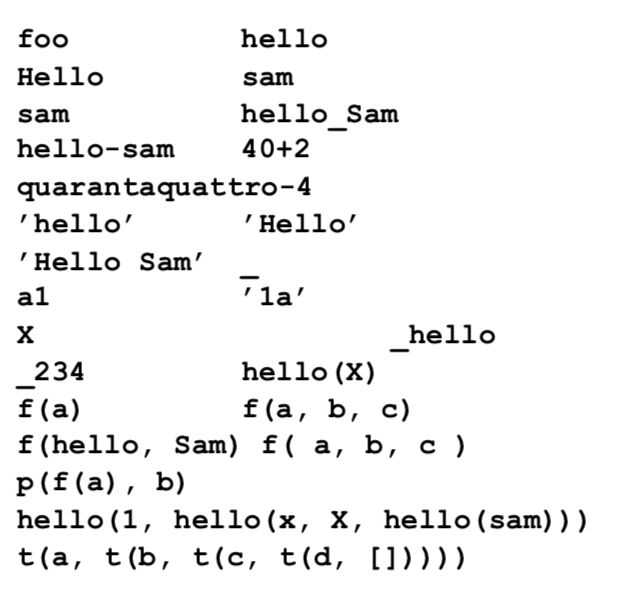
\includegraphics[width=0.75\textwidth]{validi}
\end{center}
Come si nota sono un po' di comandi a caso, ma privi di errori sintattici \\
{\color{black} \rule{\linewidth}{0.3mm} }
\\
Vediamo ora invece un esempio di comandi NON validi 
\paragraph{Non validi}
\begin{center}
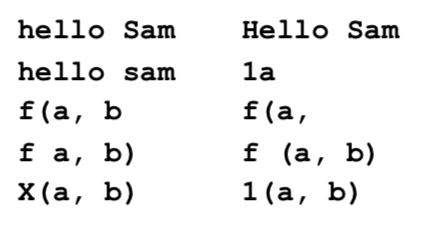
\includegraphics[width=0.75\textwidth]{nonvalidi}
\end{center}
In questo caso come vedete sono errori che tendenzialmente era possibile fare 
pure su Java, non è che si tratti di chissà che di complesso. \\
{\color{black} \rule{\linewidth}{0.3mm} }
\\ \\
\subsection{Le variabili (logiche)}
La variabile logica è una sequenza alfanumerica che però inizia con un carattere
maiuscolo (oppure con l'Underscore \_), e se son composte solo dal simbolo \_ 
prendono il nome di Indifferenza o anonime.
\\ \\
Vengono instanziate (legate ad un valore) con il procedere del programma 
(Nella dimostrazione del teorema)
\subsection{Termini Composti}
In cosa consiste una composizione di termini? In un \color{red} funtore
\color{black} (Simbolo funzione, o predicato definito come atom) +
una sequenza di termini racchiusi tra parentesi tonde e separati da virgole.
Questi ultimi sono come gli argomenti dei metodi che facevamo in java, stesso
identico concetto. \\ \\
Non serve nemmeno essere uno spazio tra funtore e parentesi di sinistra, per 
via di caratteristiche del sistema di parsing di prolog
\section{Le Regole}
Sono utilizzabili per esprimere definizioni:
\begin{itemize}
	\item Se X è un animale ed X ha le squame, X è un pesce
\end{itemize}
Ma in modo informale una regola alla fine è una formula ben formata, ed è composta
da una testa e da un corpo (collegate da un operatore) quindi per ipotesi, una 
possibile regola potrebbe essere A :- B, concettualmente si legge A è 
implicata da B.
\\ \\
La testa di una regola è il conseguente di una implicazione logica, cioè quello 
che consegue dal corpo, che è appunto l'antecedente.
\begin{lstlisting}[language = Prolog]
A :- B
\end{lstlisting} 
si può tradurre in $B \to A$, ora proviamo a ritradurre il nostro
esempio del pesce:
\begin{lstlisting}[language = Prolog]
pesce(X) :- animale(x), ha_le_squame(X)
\end{lstlisting} 
In cui la virgola ovviamente è un and ($\wedge$) \\ \\
\paragraph{Attenzione: } già questo esempio presenta una vulnerabilità, nel senso
che per intenderci, essere un pesce implica di aver le squame, MA essere un 
animale ed avere le squame non implica essere un pesce.
\section{Regole di ricorsione}
Proviamo a definire il concetto di un antenato, che è l'esempio più semplice 
per capire come funzionano le formule ricorsive. Ci conviene ancora ragionare 
sulle nostre definizioni
\begin{lstlisting}[language = Prolog]
antenato(X, Y) :- genitore(X, Y).
antenato(X, Y) :- genitore(Z, Y), antenato(X, Z).
\end{lstlisting}
Traducendolo: \\
La prima riga si legge: \textbf{SE}~~~~ X è \color{red}genitore \color{black} di Y
\textbf{ALLORA} X è \color{red}antenato \color{black} di X. \\ \\
La seconda riga invece è appena appena più complessa, merita un ritorno a capo 
solo per lei: \\ \\
\textbf{SE}~~~~ X è \color{red}antenato \color{black} di Z \textbf{E} Z 
è \color{red}genitore \color{black} di Y \textbf{ALLORA} X è \color{red}antenato
\color{black} di Y
\section{L'interprete prolog: Interrogazioni}
Come detto in precedenza possiamo chiamarle interrogazioni, query, goal, non sono
altro che comunicazioni dirette all'interprete che una volta fatto partire ci 
presenterà true o false. \\ \\
Un esempio di query:\\ 
\begin{lstlisting}[language = Prolog]
?- libro(kowalski, prolog).
\end{lstlisting}
Prolog ti restituirà come abbian detto prima true o false, yes o no, insomma ci
siamo capiti.
\\ \\
Volendo io posso interrogare anche il programma usando delle variabili esistenziali.
In pratica tutte le variabili Prolog le instanzia quando prova a darti una risposta,
e queste vengono mostrate nella tua risposta, per esempio:\\
libro(AUTORE, prolog) si legge come: CHI E' L'AUTORE DI PROLOG? 
(Un folle di sicuro, ma va be'.) \\ \\
\section{Unificazione: introduzione}
L'operazione di instanziazione di variabili durante la prova di un predicato è il 
risultato di una procedura particolare detta \textbf{Unificazione} \\ \\
Dati due termini, la procedura di unificazione crea un insieme di sostituzioni 
delle variabili, e questo insieme permette di rendere uguali i due termini. \\
\\ 
Tradizionalmente la procedura di unificazione costruisce un insieme di sostituzioni
che prende il nome di "Most general unifier (indicato con MgU)" (No, fan della F1
non c'entra nulla con l'MGU-K o H :C)
\\ \\ 
Noi non faremo unificazioni, ci pensa l'interprete Prolog, che usa le 
unificazioni appunto. L'interprete Prolog stupido, che esegue algoritmicamente
operazioni semplici, deve tenere traccia di tutte le unificazioni, quindi rinomina
le variabili che userà durante il processo,
\\ \\
Come testiamo questa cosa? Prendiamo le due espressioni che vogliamo testare, le
poniamo con il simbolo uguale in mezzo, e ci darà il risultato. Possiamo chiedergli
42 = 42? e 42=x e ci dà yes in entrambi questi casi
\subsection{Most General Unifier} 
E' il risultato finale della procedura di valutazione, o meglio, di prova del 
Prolog. \\
Il modo più comodo per vedere appunto come la procedura di unificazione funziona 
è di usare l'=
\section{Le Liste in Prolog: }
Si definisce una lista in Prolog racchiudendo gli elementi (termini e/o variabili
logiche) della lista tra parentesi quadre e si separano con le virgole.
Gli elementi di una lista in Prolog possono essere termini qualsiasi o liste. \\
$[~]$ indica la lista vuota.
\\ \\
Ogni lista non vuota può essere divisa in due parti, la testa e la coda, che sono
rispettivamente il primo elemento e "tutti gli altri". Un po' come in F1, la 
testa è la Mercedes, la coda son tutte le altre squadre (O la Juve in Serie A
negli ultimi anni).
\section{L'operatore | }
Si usa per separare e distinguere tra inizio e la coda di una lista. BONI, NON 
TRA LA TESTA E LA CODA, ma tra alcuni elementi e la nostra lista
\paragraph{Prolog lavora su strutture ad albero }, infatti i programmi sono delle
vere e proprie strutture per i dati, e sono manipolabili (mediante predicati
extra-logici, cioè che vanno oltre a quelli del programma stesso)
\\ \\
Inoltre, già detto varie volte, Prolog è un linguaggio che sfrutta la 
\textbf{Ricorsione}, in cui manca una nozione semplice di assegnamento.
\\ \\
Se con gli algoritmi si studiava il metodo di soluzione di una serie di problemi,
in questo caso ci si concentra direttamente sulla specifica del problema.
\section{La differenza tra Clausola semplice e Clausola di \color{red} Horn
\color{black}}
Una possibile clausola può essere l'implicazione: $A \to B$, che è traducibile
in $\neg(A \vee B)$ ed è leggibile in diversi modi, tutti coincidenti.
\begin{itemize}
	\item B è \textbf{implicato} da A
	\item \textbf{Se} A \textbf{allora} B
	\item A \textbf{implica} B
\end{itemize}
Se invece di esserci A e B ci fossero due insiemi di $\kappa$ e $\lambda$ 
termini avremo che:
\[
(A_{1}, A_{2}, ... ,A_{\kappa}) \wedge \neg(B_{1}, B_{2}, ... ,B_{\lambda})
\]
A e B assumono nome di \color{red} letterali \color{black}, e son positivi 
quando non presentano la negazione ($\neg$).
\\ \\
La clausola di Horn oggettivamente non è altro che una di queste clausole MA 
che ha MASSIMO, AL PIU', NON PIU' DI UN letterale positivo.
\\ 
In Prolog alla fine quel che si verifica è questo:
\begin{itemize}
	\item \color{red} Fatti:  \color{black} A. (E' il caso limite in pratica)
	\item \color{red} Regole: \color{black} A :- $B_{1}, ..., B_{n}$
	\item \color{red} Goals/Query/Interrogazioni:  \color{black} :- $B_{1}, ..., B_{n}$ \\
	Nella trasformazione di DeMorgan viene negato perchè è una clausola da 
	aggiungere, per questo si presenta con questa notazione, ma noi
	programmatori scriveremo un letterale positivo od una congiunzione di 
	letterali positivi
	\item \color{red} Contraddizioni: \color{black} fail
\end{itemize}
\section{Un programma logico}
Sì, ok, ma con questo fantasmagorico linguaggio ci si può fare almeno c = a + b?
\\ \\
Sì, si può, (ed è più semplice farlo in assembly), e si deve ragionare pensando
alla funzione "successore", che è una funzione in $N$, che consentirà di 
sviluppare un programma di questo tipo:
\begin{lstlisting}[language=prolog]
sum(0, X, X).
sum(s(X), Y, s(Z)) :- sum (X, Y, Z).
\end{lstlisting} 
's' sta per \textbf{successore}, proviamo a leggerlo (ricorsivamente): \\ \\
Il programma verrà interrogato in questo modo: \\
$\exists X$ sum(s(0), 0, X) \{X / s(0)\}
$\exists X$ sum(s(s(0)), s(0), W) \{W / s(s(s(0)))\} MA
Scritto in Prolog diventa
\begin{lstlisting}[language=prolog]
:- sum(s(0), 0, N)  {N s(0)}
:- sum(s(s(0)), 0, N)  {W s(s(s(0)))}
\end{lstlisting}
\paragraph{Spiegazione: } Il modo in cui va ragionato è ricorsivo, nel senso, 
siccome si è nel campo dei naturali si ha uno 0, un centro, ed il nostro caso
base chi è? L'elemento neutro rispetto alla somma (0). 
$\forall x \in N sum(0, X) = X$ \\ \\
Perchè ha 3 argomenti e non solo due? Semplicemente i primi due sono addendi ed 
il terzo è un risultato, nulla di che. Si legge così: \\
La somma di X + Y è uguale a Z SE la somma del successore di X + Y dà il successore di Z.
Quindi? Se ho 3 + 4 = 7, allora 4 + 4 = 8. Cioè all'atto pratico richiami per Y
volte il successore di X, che quindi chiamerà Y volte il successore di Z, e Z
diventerà la somma effettiva dei nostri X + Y.
\section{Sostituzioni}
Già dall'esempio qui sopra si nota che {W / s(s(s(0)))} e {N / s(0)} sono due
sostituzioni, ma in che senso? Praticamente ci dicono con quali valori (che 
potrebbero pure essere altre variabili) possiamo sostituire le variabili in un 
termine. \\ \\
Di solito si denota una sostituzione con questo formalismo:
\[
\sigma = \{ X_{1} / v_{1}, X_{2}, / v_{2}, ... , X_{\kappa} / v_{\kappa}\}
\]
Più nello specifico una sostituzione può essere considerata anche come 
\textit{funzione} applicabile ad un termine: $\sigma : T \to T$ dove T è l'insieme
di termini. \\ 
\paragraph{No, non è l'unico modo} è un possibile modo, di fatto basta un comando
del tipo sum(X,Y):- S is X+Y e ti fa la somma.
\\ \\
\section{Esecuzione di un programma}
Una computazione all'atto pratico è una dimostrazione (tramite le regole di 
risoluzione) del fatto che una formula sia verificabile (e che quindi sia un 
teorema).
\\ \\
Va determinata una sostituzione per le variabili della query per cui la query
segue logicamente dal programma.
Per esempio, se ho un programma \textbf{P} ed una query "$:- ~~ p(t_{1}, t_{2}, ..., t_{m}$"
(Ricordandoci sempre che la query NON è dentro al programma, o comunque non è
nel file sorgente del programma) allora: \\ \\
\[
\begin{cases}
Se ~ X_{1}, X_{2}, ..., X_{n} ~ sono ~ variabili ~ che ~ compaiono ~ in 
~ t_{1}, t_{2}, ..., t_{m} ~ \\ALLORA ~ \exists X_{1}, X_{2}, ..., X_{n} .
p(t_{1}, t_{2}, ..., t_{m}) \\	
\end{cases}
\]
Ed il nostro obbiettivo sarà quello di trovare una sostituzione del tipo:
\[
s = \{X_{1}/s_{1}, X_{2}/s_{2}, ..., X_{n}/s_{n}\}
\]
Da dove cicciano fuori queste s? Sono dei termini, per cui si ottiene che
\[
P \vdash s[p(t_{1}, t_{2}, ..., t_{m})]
\]
E P cos'è? Un programma. E un programma cos'è? Un'insieme di clausole di Horn.
Ed una clausola di Horn cos'è? E' una formula avente al più UN letterale positivo.
\\ \\
\begin{itemize}
	\item Dato un certo insieme di clausle di Horn è possibile derivare la clausola vuota
	SE ce n'è almeno senza testa. \textbf{Tradotto: } Se abbiamo una query $Q_{0}$ da
	provare
	\item Si deve dimostrare che da $P \cup {Q_{0}}$ si possa derivare la
	clausola vuota $\implies$ Sì, come al solito, mediante dimostrazioni per
	assurdo applicando il \color{red} \textbf{\textit{Magico principio di risoluzione
	}} \color{black}
\end{itemize}
Sì, ok, ma come?\\
C'è un problema di fondo: Se provassi tutte le risoluzioni possibili per ogni passo
e aggiungessi le clausole inferite all'insieme di partenza avresti un'\textbf{
ESPLOSIONE 
} combinatoria. \\ \\
Per evitarsi questo problema va adottata una strategia di soluzione che sia 
opportuna (No, ci sarà sempre tra le palle il \color{red} \textbf{\textit{Magico 
principio di risoluzione}} \color{black}, solo più vincolato. \\
\section{Risoluzione ad INPUT LINEARE (SLD)}
Prolog dimostra la veridicità o meno di una query con una sequenza di passi di
risoluzione (Sì, sequenza di passi, algoritmo, efficienza, $\Theta nLogn$) 
\\ \\
Infatti in Prolog la risoluzione avviene sempre tra l'ultima query derivata in 
ciascun passo e una una \textbf{clausola di programma}, ma non accade MAI tra
due clausole di programma o fra una clausola ed un goal derivato precedentemente.
\\ \\
\paragraph{Riassumendo: } Quello che si è appena descritto è definita \textbf{Definizione
SLD} (Selection function for Linear and Definite sentences Resolution; in cui
le "frasi lineari" sono essenzialmente delle clausole di Horn).
\\ \\
\paragraph{Esempio di risoluzione SLD}:
\begin{itemize}
	\item Partendo dalla Query $Q_{i} \equiv ~~ ?- A_{i,1}, A_{i,2}, ..., A_{i,m}$
	\item e dalla regola: $A_{r} :- ~~ B_{r,1}, B_{r,2}, ..., B_{r,m}$
	\item se esiste un unificatore $\sigma$ tale che $\sigma[A_{r}] = 
	\sigma[A_{i,1}]$ \\
	Allora si otterrà una nuova query $G_{i+1}$ tale che: 
\end{itemize}
$G_{i+1}$ si genera in pratica dal principio di risoluzione:
\begin{enumerate}
	\item $A_{r}$
	\item $\neg A_{i,1} \vee \neg A_{i,2}\vee ...\vee \neg A_{i,m}$ 
	\item $A_{i,1} \vee \neg B_{1}, \neg B_{2}, ..., \neg B_{m}$
	\item $\neg B_{1} \vee \neg B_{2} ... \vee \neg B_{n} \vee \neg A_{i,2},
	\vee \neg A_{i,3}, ..., \vee \neg A_{i,m}$
\end{enumerate}
\[G_{i+1} \equiv ~~ ?- B_{e,1}^{'}, B_{e,1}^{'}, ..., B_{e,1}^{'}, A_{e,1}^{'}, 
A_{e,1}^{'}, ..., A_{e,1}^{'} \]
E questo è solo \textbf{uno} dei passi di risoluzione eseguiti dal sistema Prolog,
in cui \begin{itemize}
\item Le $A^{'}$ e le $B^{'}$ sono risultati $\sigma[A] = A^{'}$ e 
$\sigma[B] = B^{'}$
\end{itemize}
\paragraph{Attenzione: } La scelta di unificare la \textbf{prima} sottoQuery 
$Q_{i}$ E' arbitraria (anche se comoda); Scegliere $A_{i,m} \vee A_{i,c}$ con 
$c \in [1,m]$ casuale sarebbe comunque accettato.
\paragraph{Se partissi invece dalla query}
$Q_{i} \equiv ?- ~~ A_{i,1}, A_{i,2}, ..., A_{i,m}$ e dalla regola (dal fatto) 
$A_{r}$, se esiste un unificatore $\sigma$ tale che $\sigma [A_{r}] = \sigma [A_{i,1}]$,
allora ottieni una nuova query $G_{i+1} \equiv ~~ ?- A_{e,1}^{'}, A_{e,1}^{'}, 
..., A_{e,1}^{'} $, ovvero, la nuova query ha dimensioni minori rispetto alla 
precedente, avendo m-1 sotto-query. \\ \\
Come già detto infatti nella risoluzione SLD , il passo di risoluzione avviene 
tra l'ultima query e una clausola di programma. 
\paragraph{Osservazione: } Per coloro che usano anche le slides noteranno che 
questa parte non è altro che una riscrittura delle suddette a parole di uno che
le sta studiando, per dirvi, quello che nelle slides si chiama Goal lo chiamo query,
ma quando una spiega con le slides, un velo di copiatura ci sarà sempre.\\
Che si chiami goal query o interrogazione, è sempre e comunque un teorema.
\\ \\
{\color{black} \rule{\linewidth}{0.3mm} }
\\
Come può essere il risultato finale? \\
\begin{itemize}
	\item Successo\\
	Viene generata la clausola vuota, ovvero se per n finito $Q_{n}$ è uguale 
	alla clausola vuota $Q_{n} \equiv $ :- 
	\item insuccesso finito
	se per n finito $Q_{n}$ non è uguale a :- e non è più possibile derivare un 
	nuovo \textbf{risolvente} da $Q_{n}$ ed è una clausola di programma
	\item insuccesso infinito
	Se è sempre possibile derivare nuovi risolventi tutti diversi dalla clausola
	vuota
\end{itemize}
La sostituzione di risposta è la sequenza di unificatori usati; applicata alle
variabili nei termini del goal iniziale dà la risposta finale.
\\ \\
Durante il processo di generazione di query intermedie si costituiscono delle 
varianti dei letterali e delle clausole coinvolte mediante la rinominazione di
variabili
\\ \\
Una variante per una clausola C è la clausola $C^{'}$ ottenuta semplicemente 
rinominando le variabili di C (Renaming).
\paragraph{Esempio: } 
p(X) :- q(X, g(Z)).
è equivalente alla clausola con variabili con nomi diversi: \\
p(A) :- q(A, q(B)). $\to$ Cambiando il nome delle variabili non ottieni nulla
di diverso (a meno che esse nel programma sono più volte usate, come in Java eh)
MA il codice potrebbe fare schifo da leggere.
\\ \\
Infatti possono esserci più clausole utilizzabili per applicare la risoluzione
della query corrente, nello specifico ci sono due strategie di ricerca diverse
che si possono adottare.
\begin{itemize}
	\item Depth first: (In profondità) Si sceglie una clausola e la si mantiene fissa 
	finchè non si arriva alla clausola vuota o all'impossibilità di nuove risoluzioni,
	ed in quest'ultimo caso si riconsiderano le scelte fatte in precedenza.
	\item Breadth First: (In ampiezza) Si considerano in parallelo tutte le alternative
\end{itemize}
Prolog adotta una strategia di risoluzione in profondità con \textbf{Backtracking}
cioè in pratica 
\begin{itemize}
	\item Permette risparmio di memoria MA
	\item NON è \textbf{completa} per le clausole di Horn
\end{itemize}
\section{Alberi di derivazione SLD}
Dato un programma logico P (Insieme di clausole), ed una query $Q_{0}$ con una 
regola di calcolo R, un \textbf{albero SLD} per P $\cup \{Q_{0}\}$ via R, è 
definito sulla base del processo di prova visto precedentemente
\begin{itemize}
	\item Ciascun nodo dell'albero è una query (Possibilmente vuota)
	\item La \textbf{radice} dell'albero è la query $Q_{0}$.
	\item Dato il nodo: :- $A_{1}, A_{2}, ..., A_{m-1}, A_{m}, A_{m+1}, ...,
	A_{\kappa}$, se $A_{m}$ è il sottogoal \textbf{selezionato} dalla regola di
	calcolo \textbf{R}, allora questo nodo (genitore) ha un nodo figlio per 
	ciascuna clausola del tipo: \\
	\begin{itemize}
		\item $C_{i} \equiv A_{i}$ :- $B_{i,1}, ..., B_{i,q}$
		\item $C_{\kappa} \equiv A_{\kappa}$
	\end{itemize}
	Di P tale che $A_{i}$ e $A_{m}$ ($A_{\kappa} e A_{m}$) sono unificabili 
	attraverso la sostituzione più generale $\sigma$
	\item Il nodo figlio è etichettato con la clausola goal \\
	:- $\sigma[A_{1}, ..., A_{m-1}, B_{i,1}, ..., B_{i,q}, A_{m+1}, ..., A_{\kappa}]$
	:- $\sigma[A_{1}, ..., A_{m-1}, A_{m+1}, ..., A_{\kappa}]$ \\
	E il ramo dal nodo padre al figlio si etichetta sostituendo $\sigma$ dalla
	clausola selezionata $C_{i}, C_{\kappa}$
	\item Il nodo vuoto indicato da :- non ha figli
\end{itemize}
\paragraph{Just a reminder: }La regola \textbf{R} è variabile:
\begin{itemize}
	\item Può essere scelta dalla sottoquery più a sinistra (se c'è) $\to$ Left - most
	\item Può essere scelta dalla sottoquery più a destra (se c'è) $\to$ Right - most
	\item Oppure può anche essere scelta da una sottoquery a caso
	\item Infine può essere scelta dalla sottoquery migliore
\end{itemize}
Prolog in pratica adotta la regola del Left Most, quindi considera la sottoquery
più a sinistra e l'albero SLD (implicito) generato dal sistema Prolog ordina i 
figli di un nodo secondo l'ordine dall'alto verso il basso delle regole e dei 
fatti del programma \textbf{P}.
\\
{\color{black} \rule{\linewidth}{0.3mm} }
\\
\paragraph{Illustrazione presa dalle slides}
\begin{center}
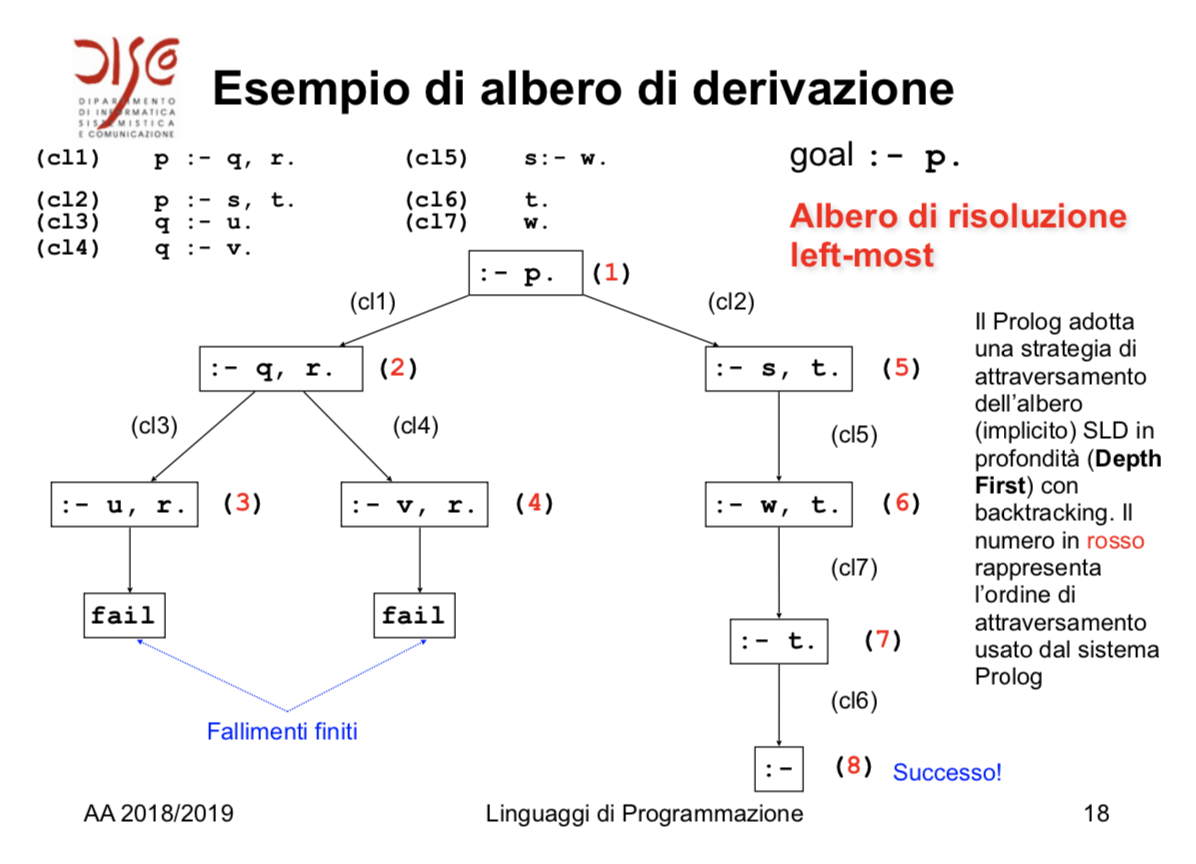
\includegraphics[width=0.75\textwidth]{alberoSLD}
\end{center}
{\color{black} \rule{\linewidth}{0.3mm} }
\\
Cerchiamo di ragionare bene sull'albero visto nell'esempio qui sopra. Abbiamo
una serie di clausole, sono le varie cl1, 2, 3, ..., 7. Ora, quello che accade
è che da sinistra verso andiamo ad applicarle alla clausola principale.
\\ \\
Non so se è stato già detto, tutto questo casino è semplicemente quello che 
effettua Prolog per quando dimostra un teorema \\ \\
Quindi quel che si verifica è proprio che si hanno due fail, e chiudiamo 
poi con una clausola vuota (:-) quindi quello che concludiamo è che tutto è 
andato a buon fine.
\paragraph{Stesso esercizio MA con tecnica Right-Most fatto da} 
\href{https://github.com/LiaBell47}{Giulia}
\begin{center}
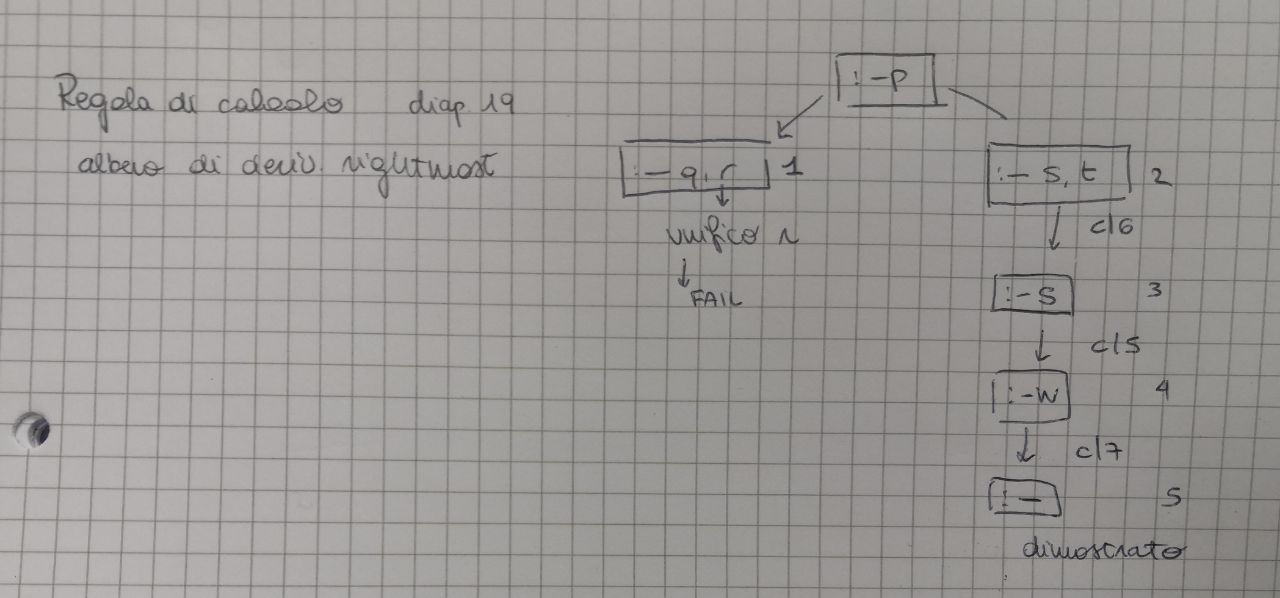
\includegraphics[width=0.80\textwidth]{rightmost}
\end{center}
{\color{black} \rule{\linewidth}{0.3mm}}
\\
\paragraph{Immagine tratta dalle slides}
\begin{center}
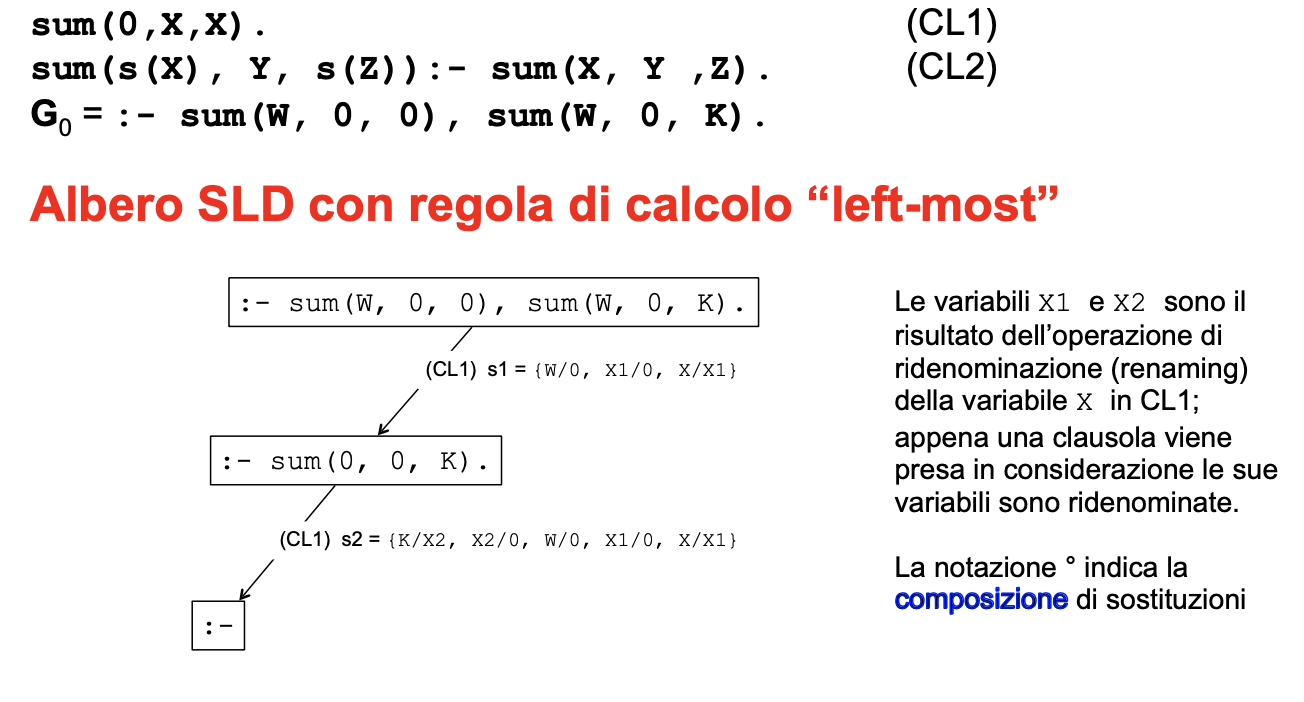
\includegraphics[width=0.75\textwidth]{8}
\end{center}
L'esercizio è giusto se per ogni passaggio si specifica quale clausola si usa,
con i dati ad essa collegati come in questo esempio. \\  \\
Nel primo passaggio usiamo solo la clausola 1 perchè la clausola 2 non era 
applicabile. 
\\
{\color{black} \rule{\linewidth}{0.3mm}}
\begin{center}
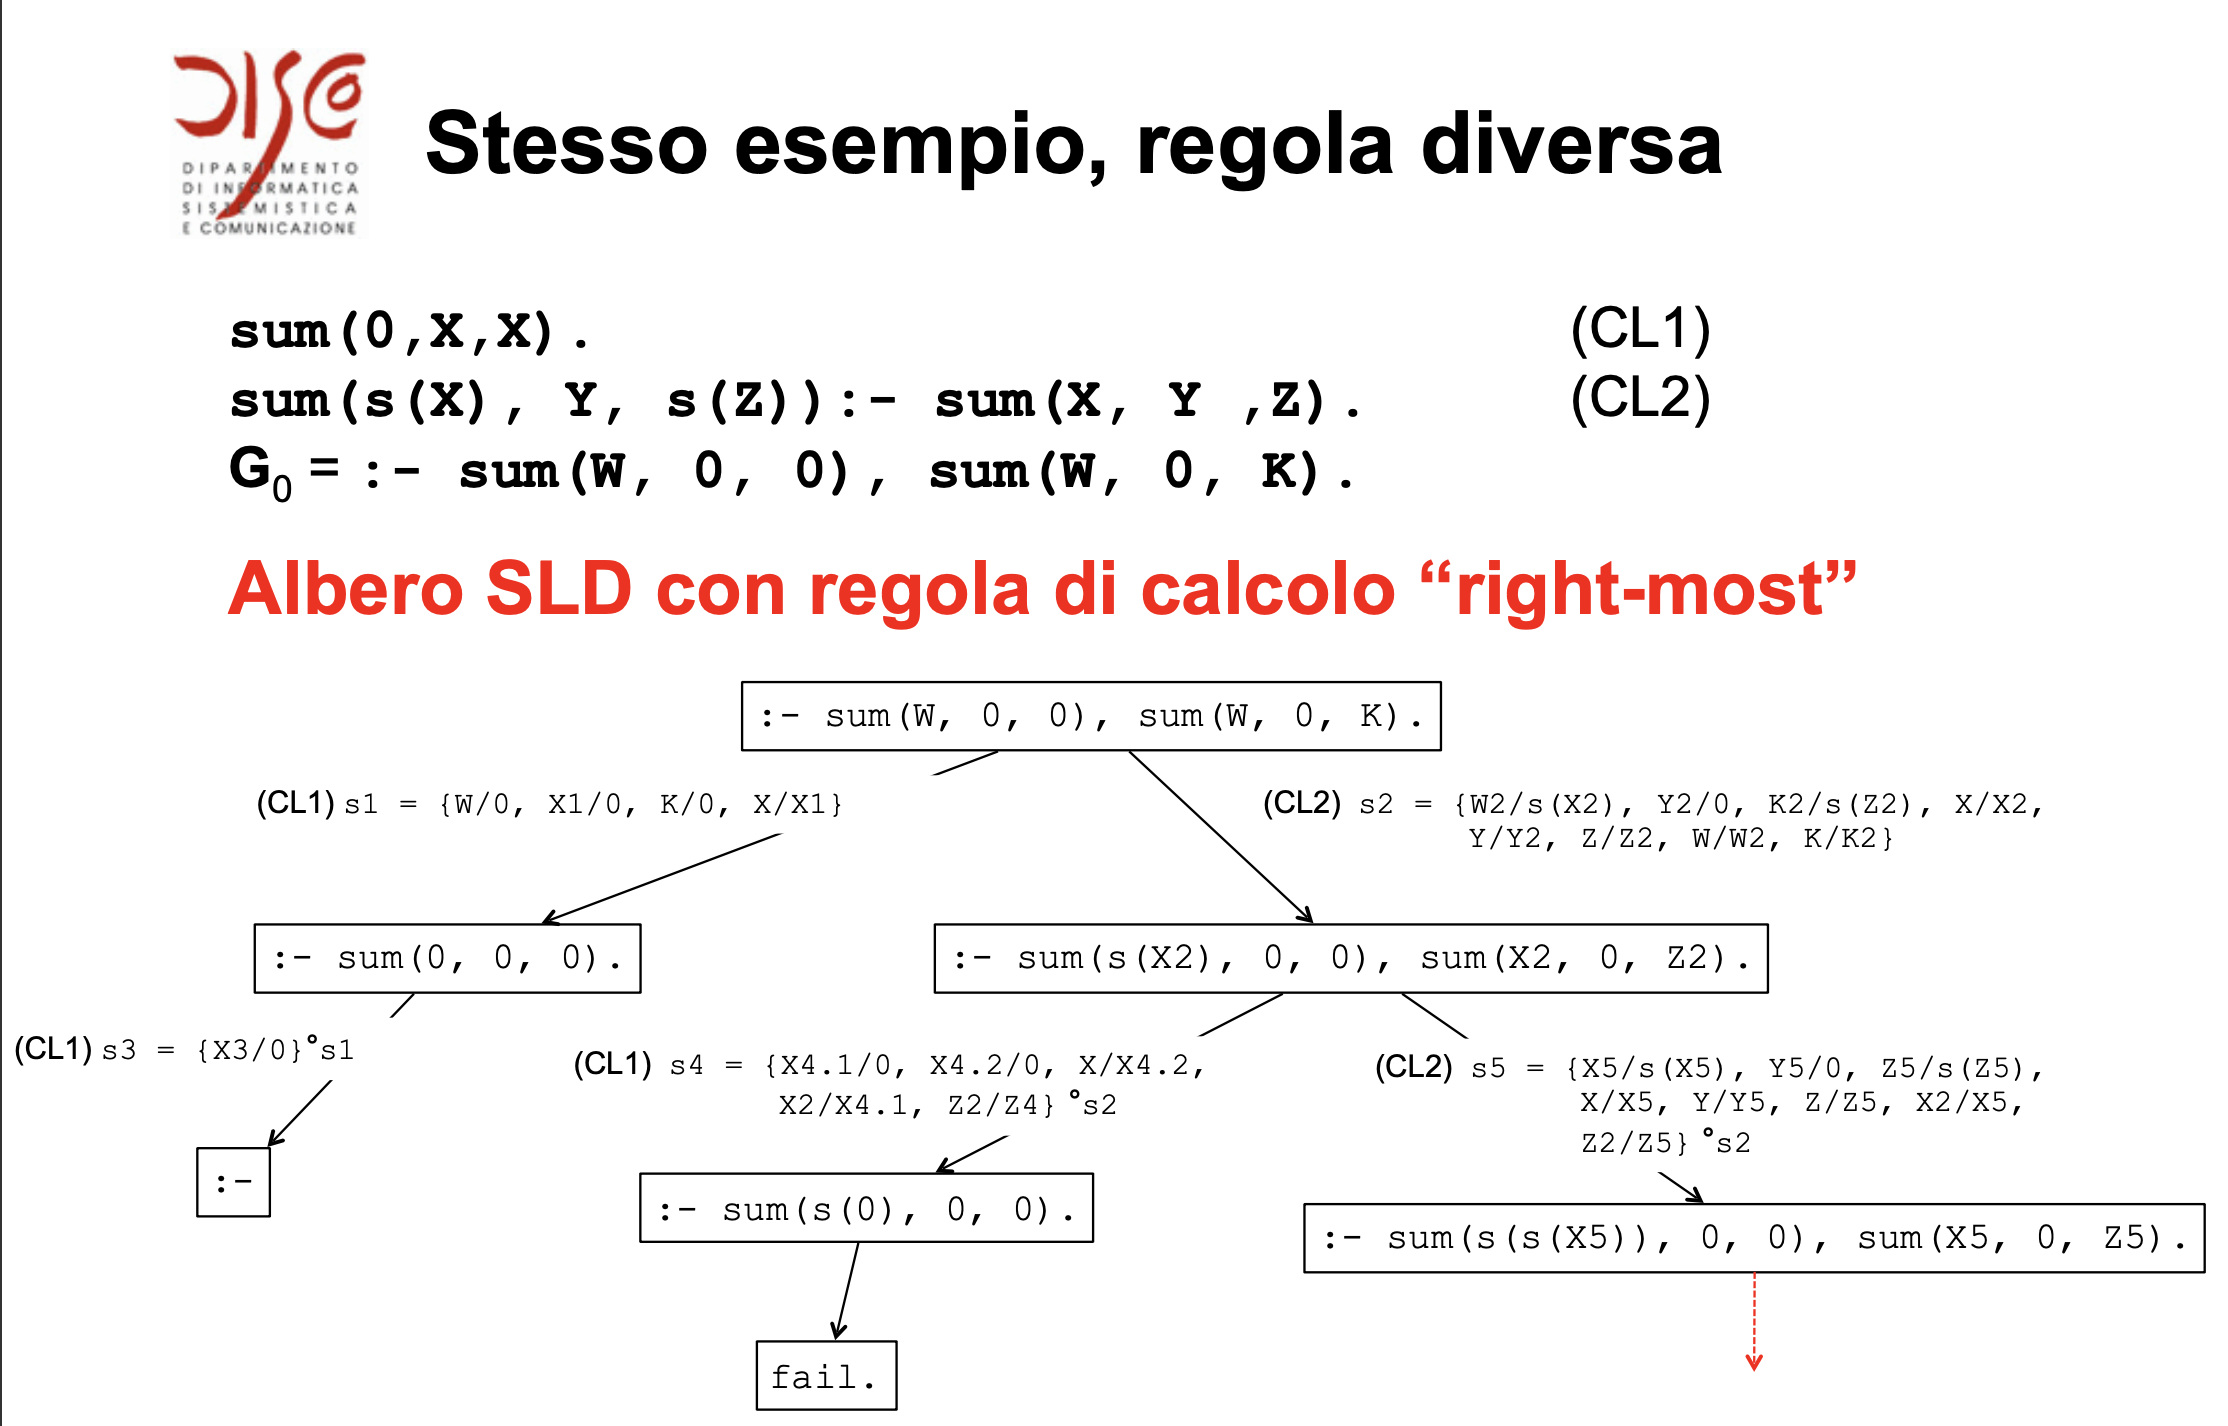
\includegraphics[width=0.75\textwidth]{9}
\end{center}
In questo caso abbiamo costruito prima da sinistra poi da destra, MA c'è da
considerare che Prolog ragiona Left-Most, ANCHE SE al compitino è possibile
comunque decidere il metodo di lavoro.
\section{La regola di calcolo}
Per ogni ramo di un albero SLD corrisponde una derivazione SLD. In pratica ogni 
ramo che termina con il nodo vuoto (:-) \\ \\
La regola di calcolo influisce sulla scrittura dell'albero per quanto concerne
sia l'ampiezza che la sua profondità \\ \\
La cosa che va garantita è che tutti i cammini di successo siano uguali 
concettualmente, (la parola regola si incontra per l'ennesima volta tra l'altro, 
prima son state la regola di inferenze e la regola di Prolog) \\ \\
Perciò alla domanda "quante accezioni del concetto di regola sono state 
menzionate", si risponderà: 3
Le regole di calcolo \color{red} NON \color{black} influisce su \color{red} 
correttezza \color{black} e \color{red} completezza \color{black}, pertanto 
qualunque sia R, il numero di cammini di successo (se finiti obv) è lo stesso
in qualsiasi albero SLD costruibile per $P \cup \{G_{0}\}$
%-------------------------------------------------------------------------------
\chapter{Modello di esecuzione Prolog}
Come lavora effettivamente Prolog con le dimostrazioni?\\

Prendiamo ora per esempio \[p~:-~q,~r.\](E rispettiamo questi spazi, quindi 
graficamente dovrà proprio essere considerata così) E' possibile dare più di una
interpretazione a questa formula:
\begin{enumerate}
	\item Interpretazione dichiarativa\\
	p è \color{red}vera se  \color{black}sono veri q ed r
	\item Interpretazione procedurale\\
	p è scomponibile in due sottoproblemi (q ed r)\\
	{\color{black} \rule{\linewidth}{0.3mm}}
	\paragraph{Immagine tratta dalle slides}
	\begin{center}
	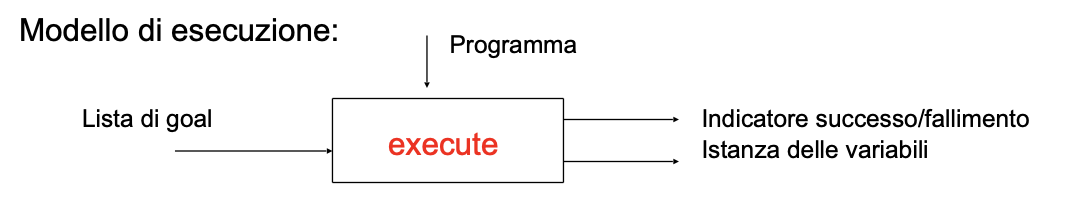
\includegraphics[width=0.75\textwidth]{2}
	\end{center}
	Da quest'immagine possiamo definire alcune cose:
	\begin{enumerate}
		\item Un goal può essere visto come una chiamata ad una procedura
		\item Una regola può essere vista come definizione di una procedura in
		cui la testa è l'intestazione mentre la parte di destra è il corpo.
	\end{enumerate}
	{\color{black} \rule{\linewidth}{0.3mm}}
\end{enumerate}
\section{Le Estensioni}
Per rendere Prolog un linguaggio che abbia senso essere usato si aggiungono le
notazioni per le liste e meccanismi per il caricamento del codice Prolog,
\color{red} \textbf{MA NON SOLO} \color{black}, si introducono anche le seguenti
funzioni da "vedere":
\begin{itemize}
	\item Meccanismi di controllo del backtracking
	\item Operazioni aritmetiche ($+~-~*~/$)
	\item Trattamento della negazione
	\item Possibilità di manipolare e confrontare le strutture dei termini
	\item Predicati meta ed extra-logici
	\item Predicati di I/O
	\item Meccanismi per modificare/accedere alla base di conoscenza
\end{itemize}
\section{Il controllo di flusso}
Se un sottoGoal fallisce, il dimostratore di Prolog sceglie un'alternativa 
procedendo in sequenza dall'alto verso il basso della lista O MEGLIO, dalla 
testa alla coda della lista delle clausole. \\ \\
Però Prolog mette a disposizione il "\textbf{cut}", che non è altro che un 
taglio, che si indica con un '\textbf{!}', che serve per controllare questa
megaEnormeListona di scelte.\\ \\
\subsection{Caratteristiche del Cut}
Ha un problema di fondo, ovvero il fatto che è complesso da interpretare, perchè
non ha un'interpretazione logica, ma procedurale. \\ \\
Inoltre per capire come funziona serve conoscere meglio il funzionamento del 
dimostratore Prolog, che esegue su una macchina virtuale (SI'! Proprio come Java!)
\\ \\
Neanche a dirlo, la sua importanza non è sottovalutabile, se no che lo 
studieremmo a fare?
\section{Il predicato '!' (Cut)}
Per capire meglio il funzionamento di questo predicato serve scriverci una
clausola generica (avente il cut, e grazie al.. No, non mi abbasserò a tal
livello da dire "cut"). 
\[
C = a :- b_{1}, b_{2}, ..., b_{\kappa} !, b_{\kappa + 1}, ..., b_{n}.
\] 
Cerchiamo di procedere con ordine, cosa fa questo cut?\\
In pratica se il goal corrente G unifica con a e $b_{1}, b_{2}, ..., b_{\kappa}$
hanno successo ALLORA il dimostratore 
si impegna inderogabilmente alla scelta di C per dimostrare G \\ \\
Ogni clausola alternativa (sì, quelle che si scorrono dall'alto verso il basso, 
quindi sarà quella dopo) per a che unifica con G viene ignorata\\ \\
\paragraph{ATTENZIONE: } Per un qualche $b_{j}$ con $j > \kappa$ fallisse, 
allora il backtracking si fermerebbe ai cut
(Le altre scelte per i $b_{i}$ con $i \leq \kappa$ vengono rimosse, cancellate,
e rimosse dall'albero di derivazione). \\ \\
Inoltre, se il backtracking raggiunge il cut, automaticamente lui fallisce, e la
ricerca procede dall'ultimo punto di scelta prima che G scegliesse C.
\paragraph{Ragioniamo sul seguente codice:}
\begin{center}
cl1: a ~ :- ~ p,~ b. \\
cl2: a ~ :- ~ p,~ b. \\
cl3: p.
\end{center}
In cui cl indica la clausola, e considereremo la query "?- a.", Questo sarà
lo stato interno di Prolog
\\
{\color{black} \rule{\linewidth}{0.3mm}}
\paragraph{Immagini tratte dalle slides}
\begin{center}
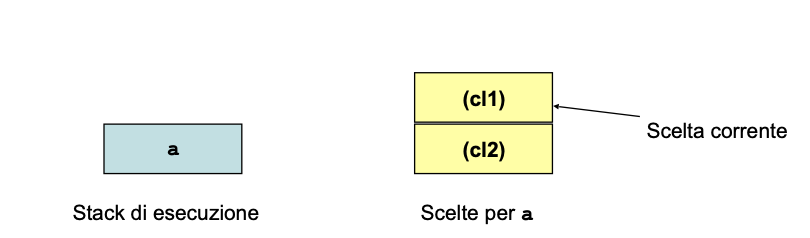
\includegraphics[width=0.75\textwidth]{3}
\end{center}
Nel momento in cui chiedo di dimostrare il seguente problema Prolog mi genera
due stack, uno di esecuzione in cui si memorizza il goal corrente, mentre 
l'altro contiene le clausole unificanti \\
In pratica quello che accade è che p viene messa in cima allo stack
\begin{center}
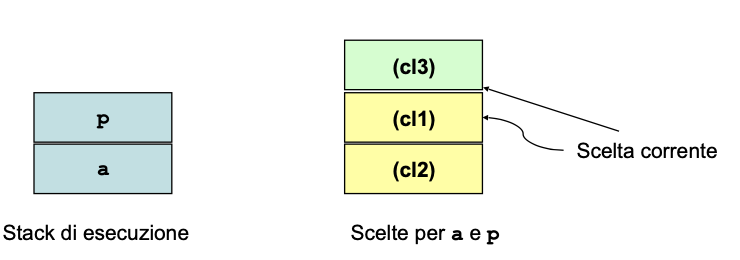
\includegraphics[width=0.75\textwidth]{4}
\end{center}
Se per ipotesi p ha successo, si inserisce b in cima allo stack\\
Se in questo caso la valutazione di b fallisce, si attiva il meccanismo magico
del \color{red} backtracking \color{black} e quindi per proseguire si passa a
considerare la seconda clausola, e lo stato interno di prolog cambia. \\
Come cambia?
\begin{center}
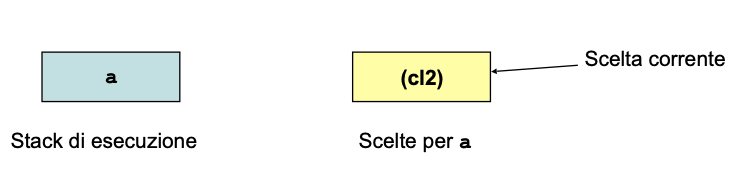
\includegraphics[width=0.75\textwidth]{5}
\end{center}
Quello che accade ora è che p si mette in cima allo stack, ha successo, MA
la valutazione di c fallisce, perciò di nuovo backtracking, però attenzione,
siccome non ci sono più clausole allora anche a fallisce, e lo stack si svuota.
\\ \\
Analizziamo meglio però questi stack (queste pile)
\begin{itemize}
	\item Pila di esecuzione: \\
	Contiene tutti i record di attivazione delle varie procedure (sostituzioni
	per unificare le varie regole)
	\item Pila di \color{red}\textbf{backtracking} \color{black} che contiene 
	l'insieme dei "punti di scelta". Ad ogni fase della valutazione semplicemente
	contiene dei puntatori alle scelte "aperte" nelle fasi precedenti della
	dimostrazione.
\end{itemize}
\paragraph{Cosa succede alle queries con il Cut?}
\section{I tipi di Cut}
Sono fondamentalmente 2, o meglio, sono due \textbf{USI} diversi, del predicato
cut, il predicato rimane lo stesso:
\begin{itemize}
	\item \color{green}\textbf{Green Cut: }\color{black} Utile per eseprimere 
	"determinismo" (e quindi pre rendere più efficiente il programma)
	\item \color{red}\textbf{Red Cut: }\color{black} Usati solo per efficienza,
	perchè i pratica omettono alcune condizioni esplicite e modificano la 
	semantica del programma equivalente senza i cuts (Sono indesiderabili anche
	se una volta ogni 10 anni, utili.. forse.)
\end{itemize}
\paragraph{Vediamo un esempio: }Consideriamo un programma che deve fare il merge
di due liste ordinate: 
\begin{lstlisting}[language=Prolog] 
merge([X|Xs, [Y|Ys], [Z|Zs]) :- X < Y,
merge(Xs, [Y|Ys], Zs).

merge([X|Xs, [Y|Ys], [Z|Zs]) :- X = Y,
merge(Xs, Ys, Zs).

merge([X|Xs, [Y|Ys], [Z|Zs]) :- X > Y,
merge([X|Xs], Ys, Zs).

merge([], Ys, Ys).
merge(Xs, [], Xs).
\end{lstlisting} 
\paragraph{Altro esempio: }Consideriamo un programma che serva a ricontrollare 
quale è il minimo tra due numeri:
\begin{lstlisting}[language=Prolog] 
minimo(X,Y,Z) :- X=<Y
minimo(X,Y,Y) :- Y>X
\end{lstlisting} 
Ora supponiamo di avere una query del tipo: merge([1,3,5],[2,3],Xs), qualli che
saranno i passaggi saranno i seguenti:
\begin{enumerate}
	\item merge([1,3,5],[2,3],Xs).
	\item 1 < 2: merge([3,5],[2,3],Xs1).
	\item 3 < 2: merge([3,5],[2,3],Xs1). FALLISCE, si fa backtracking al passaggio
	2
	\item 1 = 2: merge([3,5],[2,3],Xs1). FALLISCE, ancora backtracking al passaggio
	2
	\item 1 > 2: merge([3,5],[2,3],Xs1).
\end{enumerate}
Solo una clausola avrà successo, le altre non verranno considerate.
\paragraph{Altro possibile problema con Prolog} (L'ennesimo dei tanti). Se per
ipotesi si avesse una query di questo genere: 
\begin{lstlisting}[language=Prolog] 
?- merge([],[],Xs).
\end{lstlisting} 
Quando noi andremo effettivamente a visualizzare i possibili valori della variabile
Xs, prolog ci risponderà due volte con Xs = []. Si ha una soluzione in più, c'è
ridondanza. Il green cut risolve questo specifico problema.
\paragraph{Determinismo: }
\subparagraph{Per definizione: }
Un programma Prolog si dice deterministico quando una sola delle clausole serve 
(o si vorrebbe servisse) per provare un dato goal. \\ \\

Un programma sviluppato in Prolog si dice deterministico, ovvero, si ha una 
corrispondenza tra i dati di input e l'output effettivo. Non si ha questa 
ridondanza insomma, il codice diventerebbe così:
\begin{lstlisting}[language=Prolog] 
merge([X|Xs, [Y|Ys], [Z|Zs]) :- X < Y,
merge(Xs, [Y|Ys], Zs), ! .

merge([X|Xs, [Y|Ys], [Z|Zs]) :- X = Y,
merge(Xs, Ys, Zs), ! .

merge([X|Xs, [Y|Ys], [Z|Zs]) :- X > Y,
merge([X|Xs], Ys, Zs), ! .

merge([], Ys, Ys) :- !.
merge(Xs, [], Xs) :- !.
\end{lstlisting} 
Invece per quanto concerne la funzione del minimo:
\begin{lstlisting}[language=Prolog] 
minimo(X,Y,X) :- X =< Y, !.
minimo(X,Y,Y) :- Y < X, !.
\end{lstlisting} 
In pratica il green cut taglia le strade che NON verrebbero comunque ad avere
successo. Perchè se una strada ha successo, le altre non ha senso provarle. 
Se vogliamo essere pignoli, il secondo cut è ridondante MA per ragioni di 
simmetria viene messo nel programma. 
\section{Il \color{red}Red cut\color{black}}
Lo stesso programma potevamo scriverlo in un modo ancora più sintetico:
\begin{lstlisting}[language=Prolog] 
minimo(X,Y,X) :- X =< Y, !. 
minimo(X,Y,Y).
\end{lstlisting} 
Come vedete in questo caso manca tutta la condizione, ma si taglia proprio
la soluzione. Ed è talmente intelligente che se gli spariamo la query
minimo(2,5,5). (Tradotta sarebbe: E' 5 minore di 2?) ci dà TRUE! Geniale!
\paragraph{E' instabile: }Già da qui si capisce che non sia corretto il programma
sia scritto scorretto, e attenzione 
\subparagraph{E' SEMPRE COLPA DEL PROGRAMMATORE: }Non è inutilizzabile, 
non è il cut in sè, è semplicemente complesso da capire ed usare. Non è sempre
ovvio quando può fallire
\chapter{Altri elementi di Prolog}
\section{Predicati Meta-Logici}
La domanda è: Perchè?\\
Consideriamo il seguente predicato:
\begin{center}
celsius\_fahrenheit(C, F) :- C is 5/9 * (F - 32).
\end{center}
Non è \color{red}invertibile  \color{black} ed introdurre la seconda clausola
\begin{center}
celsius\_fahrenheit(C, F) :- F is (9/5 * C) + 32.
\end{center}
non aiuta, perchè il sistema già sulla prima clausola si blocca.\\ \\
Il problema sta nel decidere chi fa l'\textbf{inout} e chi invece l'\textbf{output}
del calcolo. \\ \\
Qua non è che ti dà il \textit{fail} ma letteralmente ti dà errore. E quindi
che si può fare? La risposta è nel titolo di questa sezione, ovvero, usare
i predicati meta-logici. \\ \\
Più precisamente però, cosa sono? Allora, abbiamo alcuni predicati NON 
invertibili (minimo, celsius\_fahrenheit), e questo accade a causa dell'uso che
abbiamo applicato dei predicati aritmetici dei predicati (>, <, $\leq$, 
\textbf{is}, etc). \\ \\
I meta-logici sono predicati che danno un valore agli elementi delle nostre forme,
fondamentalmente prendono le variabili, e le usano come oggetti del linguaggio,
in modo da effettuare alcune scritture che aiutano a comprendere la semantica.
%
\paragraph{Mi spiego peggio: } Prendete un'espressione del tipo variabile(X), 
che tradotto è "X è una variabile", bene, il predicato meta-logico è quello 
che definisce per esempio notVariabile(X)\\ \\
Tutto ciò è inseribile nel corpo delle nostre regole, è quello il motivo del
perchè i predicati metalogici assumono molta importanza.
\paragraph{Riprendendo l'esempio di prima:}
\begin{center}
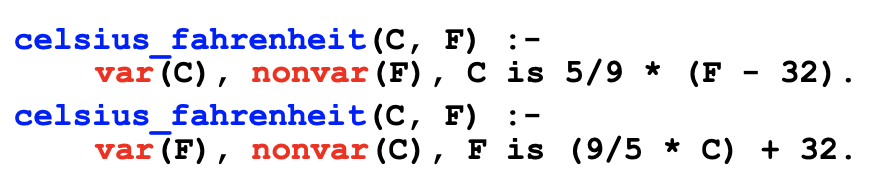
\includegraphics[width=0.75\textwidth]{6}
\end{center}
L'uso di var(X) permette di capire quale clausola usare! Cosa se ne ricava? Che
l'uso di questi predicati magici consente di scrivere dei programmi efficienti 
ED allo stesso tempo corretti semanticamente. \\ \\
Bene, ma se C ed F fossero entrambe variabili? Scritto così il programma ragiona
che SE C è variabile esegue il primo blocco ALTRIMENTI il secondo, ma se fossero
entrambe delle variabili?  
\paragraph{Risposta: } I due "if" sono se una è variabile e l'altra no, ALLORA 
fai cose, ma non è implementato SE entrambe son variabili o costanti, darebbe
errore. Per intenderci, è uno XOR\\ \\
Nel senso: Se la query fosse: celsius\_fahrenheit(X, Y)? Possiamo usare dei cut
per scrivere un programma più completo??
\section{Ispezione di termini}
Finora abbiamo visto come si usano dei termini per rappresentare strutture per i
dati, ed abbiamo inoltre intuito che esistono termini atomici e composti, ed 
ora vedremo come implementare tutto ciò in Prolog:
\begin{itemize}
	\item atomic(X): SE x è un numero od una costante ALLORA true
	\item compound(X): SE non atomic(X) ALLORA true
\end{itemize}
A questo punto, consideriamo un termine \textbf{Term}, ci saranno ben tre
predicati che tornano utili per manipolarlo:
\begin{enumerate}
	\item \color{red}functor \color{black} (Term, F, Arity)\\
	vero se Term è un termine, con Arity argomenti, il cui funtore (simbolo di 
	funzione o di predicato) è F
	\item \color{red}arg \color{black} (N, Term, Arg)\\
	Ritorna l'ennesimo argomento del termine, o meglio, è vero SE l'ennesimo 
	argomento di \textbf{Term} è \textbf{Arg}
	\item Term =.. L\\
	Questo è il più complesso, bisogna capirci bene a fondo, perchè qua si ha 
	un predicato che è "=..", è un predicato binario di cui uno è termine ed
	uno è la lista. \\ \\
	Nei termini del linguaggio universale si chiama anche \textbf{univ}. 
	\paragraph{Ma cosa fa questo predicato?} Prende un termine e lo trasforma
	in una lista, ed il primo elemento sarà il funtore, e tutti gli altri 
	saranno semplici argomenti, in questo modo si appiattisce tutto. Diventa 
	Lista = $argomento_{1}, argomento_{2}, ..., argomento_{\lambda}$
\end{enumerate}
\section{Predicati di ordine superiore}
Quando si formula una domanda a Prolog, ci si aspetta una risposta (che poi
alla fine non è altro che istanza individuale derivabile).
Di fatto il backtracking come abbiamo visto ci permette di estrarre tutte le 
istanza derivabili una alla volta.\\ \\
Ma se volessimo come risultato l'insieme di tutte le istanze che soddisfano una
certa query?\\ \\
Questa non è una richiesta associabile alla logica del primo ordine, noi ora
si sta facendo una domanda in cui X si associa ad un insieme, e quest'idea di 
assegnare ad una variabile un insieme è quello che distingue la logica del secondo
ordine dal primo.\\ \\
Nella logica del primo ordine un elemento va ad un elemento, nel secondo ordine 
una variabile va ad un insieme, è un po' diverso insomma.
\textbf{Prolog} mette a disposizione una serie di \textbf{Predicati su Insiemi}
che \textbf{estendono} il \color{red}modello  \color{black} computazionale
del linguaggio di base.
\section{Predicati su Insiemi}
Sono fondamentalmente 3:
\begin{enumerate}
	\item \color{red}\textbf{findall} \color{black} (Template, Goal, Set):\\
	E' un predicato di arità 3, forse non è chiaro da questa sintassi, ma l'idea
	di fondo è: \\ \\
	Noi abbiamo un template, che è una variabile, ma può essere pure qualcosa di 
	più complesso, una lista di oggetti, un oggetto, e come funziona? 
	\begin{itemize}
		\item SE \textbf{set} contiene \color{red}tutte \color{black} le istanze
		di \textbf{Template} che soddisfano \textbf{Goal} ALLORA vero
		\item Le istanze di \textbf{Template} vengono ottenute tramite 
		\color{red}\textbf{Backtracking}  \color{black}
	\end{itemize}
	\item \color{red}\textbf{bagof} \color{black} (Template, Goal, Bag):\\
	Ha una semantica che matematicamente si chiama BagSemantic, non è un insieme
	ma un multi-insieme, e funziona così:
	\begin{itemize}
		\item SE \textbf{bag} contiene tutte le alternative di \textbf{Template}
		che soddisfano il \textbf{Goal} ALLORA restituisce true
	\end{itemize}
	Le alternative fondamentalmente vengono costruite facendo backtracking, solo se
	vi sono delle variabili libere nel \textbf{Goal}, che non appaiono in
	\textbf{Template}\\ \\
	Inoltre si pulò pure dichiarare QUALI variabili non vanno considerate libere 
	per dire che non si vuole fare backtracking rispetto a queste ultime, 
	variabili di tipo esistenziale (si indicano con $var^{G}$)
	\item \color{red}\textbf{setof} \color{black} (Template, Goal, Set):\\
	Si comporta esattamente come \textbf{bagof} MA \textbf{set} non contiene 
	soluzioni duplicate, semplicemente
\end{enumerate}
Prolog ci mette a disposizione anche altri predicati di ordine superiore, buona
parte di questi funziona grazie al meccanismo delle meta-variabili, ovvero 
variabili interpretabili come query\\ \\
Un esempio tipico è il predicato \textbf{chiama} che si può pensare essere
definito come: \color{red} \textbf{chiama}  \color{black}(G) :- G \\
In \href{https://swish.swi-prolog.org/}{Swi-Prolog} esiste un predicato che si
chiama \textbf{call}, che fa questo \\ \\
Grazie a queste meta-variabili, possiamo definire il predicato \textbf{Applica}
che valuta una query composta da un funtore e da una lista di argomenti
\begin{center}
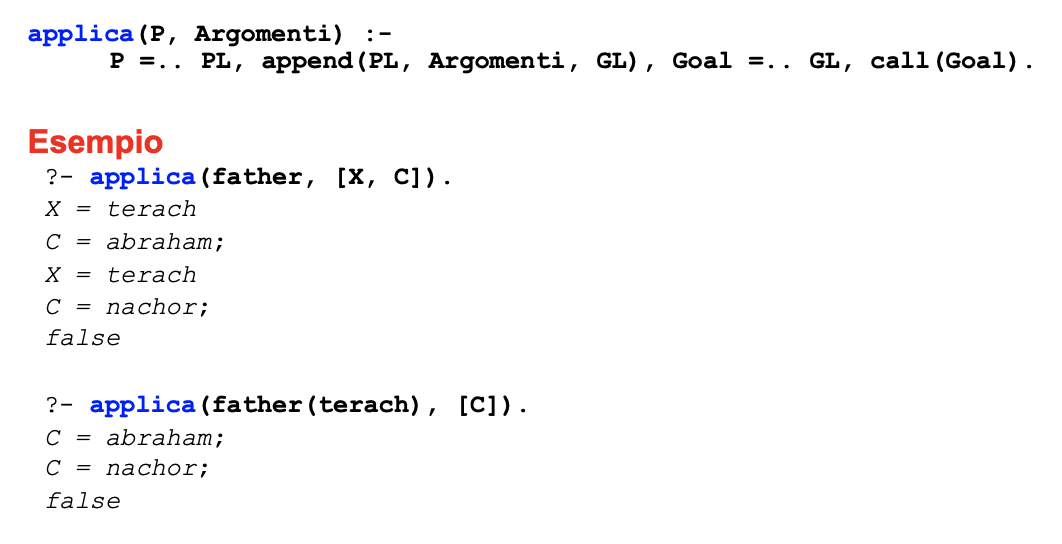
\includegraphics[width=0.75\textwidth]{7}
\end{center}
\section{Manipolazione della base di dati}  
\paragraph{Perchè manipolare direttamente la base di conoscenza? }E' di base 
una cosa utile il fatto di poter manipolare un database, soprattutto se si tiene
in mente il fatto che diventa possibile memorizzare risultati intermedi di una
computazione. (Memorization o catching)
Dato un programma Prolog, sappiamo che questo è praticamente costituioto da un
database (per favore, chiamatelo knowledge base, basi di dati è al prossimo 
semestre) contenente fatti e regole\\ \\
Il Prolog però mette a disposizione anche altri predicati che servono a 
manipolare direttamente la base di dati. Ovviamente, questi predicati vanno 
usati con molta attenzione, dato che modificano dinamicamente lo stato del 
programma.\\ \\
I suddetti predicati sarebbero:
\begin{enumerate}
	\item Listing
	\item Assert, asserta, assertz
	\item retract
	\item abolish
\end{enumerate}
Consideriamo come base il caso in cui si ha una Knowledge Base vuota 
($ \varnothing $), se interroghiamo Prolog con listing. lui ci risponderà sì.
\paragraph{Hey Prolog, mostrami la mia KB! }Sì! *Prolog left the server*\\
Più o meno è quello che accade visto che non ha nulla da mostrare.
\paragraph{Se consideriamo un assert} del tipo 
\textbf{assert(meravigliosa(firenze))}, lui ritornerà \textit{true}, come giusto
che sia! Scherzi a parte, l'assert è un comando che ha \textbf{SEMPRE} successo,
però attenzione, non è per via del suo essere praticamente una masterball dei
comandi l'importante, ma è il come può cambiare lo stato del nostro Database.
\paragraph{Riproviamo listing: } ora verrà restituito il nostro assert di prima
e un true:
\begin{lstlisting}[language=Prolog] 
?- listing.
meravigliosa(firenze).
true
\end{lstlisting} 
Riassunto, l'assert gli ha iniettato una verità assoluta, che lui accetta a 
prescindere, paradossalmente se gli ripassiamo due volte lo stesso assert, lui 
lo prende di pacco, così come glielo diamo e lo riaggiunge al database.
\paragraph{Mi spiego peggio: } Se passo a Prolog assert(bello(dave)), per due 
volte, lui quando farò il listing mi dirà:
\begin{lstlisting}[language=Prolog] 
?- listing.
bello(dave).
bello(dave).
true
\end{lstlisting} 
E se lo dice Prolog, allora è proprio vero!
\subsection{Asserzione di regole}
Ciò che abbiamo appena visto non è altro che un'asserzione di \textbf{fatti}, ma
come da titolo di questa sezione, è possibile asserire anche \textbf{regole}.
\paragraph{Esempio: } Supponiamo di voler inserire una regola che dica che 
chiunque passa LP sia felice (E beati loro):
\begin{lstlisting}[language=Prolog] 
?- assert(felice(X) :- passatoLP(X)).
bello(dave).
bello(dave).
true
\end{lstlisting} 
\paragraph{Precisazione: }Per essere risucito a scrivere questa cosa in modo 
corretto ringrazio RC per la correzione. Ho fatto l'errore di ragionare come 
se :- si traducesse in "Implica" MA NON E' COSI'. Quel simbolo è traducibili in 
"E' implicato".
\section{Varianti dell'assert}
\subsection{Asserta}
Sarebbe Assert-a, ovvero l'asserzione viene messa in cima alla lista delle 
clausole
\subsection{Assertz}
Stesso discorso dell'assert-a ma in questo caso invece di inserire all'inizio
te lo aggiunge alla fine in coda
Ora indubbiamente abbiamo asserito delle verità assolute e dimostrabili, come
la magifica bellezza di Dave MA, supponiamo che per sbaglio qualcuno asserisca
una clausola che dopo non servirà più, come si può eliminare? 
\section{Retract}
Il retract è l'operatore inverso dell'assert, molto semplicemente rimuove delle
clausole dalla lista. Per intenderci, è l'operatore PERFETTO per clausole tipo:
\begin{center}
carbonara(X, Y), ingredienti(parmigiano, Y). 
\end{center}
Che tradotto è: LA CARBONARA E' SACRA.
\paragraph{Il listing} produrrà una lista che chiaramente sarà priva della 
clausola che abbiamo rimosso (E grazie al *\textit{censura}*). \\ \\
Ad ogni modo è un comando che tornerà utile se abbiamo asserito più volte
la stessa clausola, perchè non elimina ricorsivamente tutte le occorrenze.
\subparagraph{Mi spiego peggio: }Se avessimo due volte la stessa clausola 
(felice(personaGenerica)), e volessimo rimuoverle entrambe, non sarebbe possibile.
Se ne rimuove solo una alla volta.
%\paragraph{Vediamo un esempio: } dato il codice:
%\begin{lstlisting}[language=Prolog]
%	%Versione DETERMINISTICA
%	elemento(X, [X|_]) :- ! .
%	elemento(X,[Y|Ys]) :- (X\=Y), el(X,Ys).
%
%	%Versione NON DETERMINISTICA
%	elemento4(X, [X|_]) :- ! .
%	elemento4(X, [X|_]).
%	elemento4(X,[Y|Ys]) :- (X\=Y), el(X,Ys).
%\end{lstlisting}
\chapter{Input/Output in Prolog}
Come ogni comando visto finora questi saranno predicati, che avranno la 
possibilità di acquisire e stampare valori (read, write). 
Inoltre sono presenti anche comandi di gestione di file e degli stream (open, 
close, seek etc.)
\section{Read \& Write}
Con Read e Write è possibile stampare e leggere dei \textbf{termini} Prolog,
con il write che sarebbe l'equivalente del toString() in Java, mentre read
invoca il parser di Prolog, vediamo alcuni esempi presi dalle slides:
\begin{center}
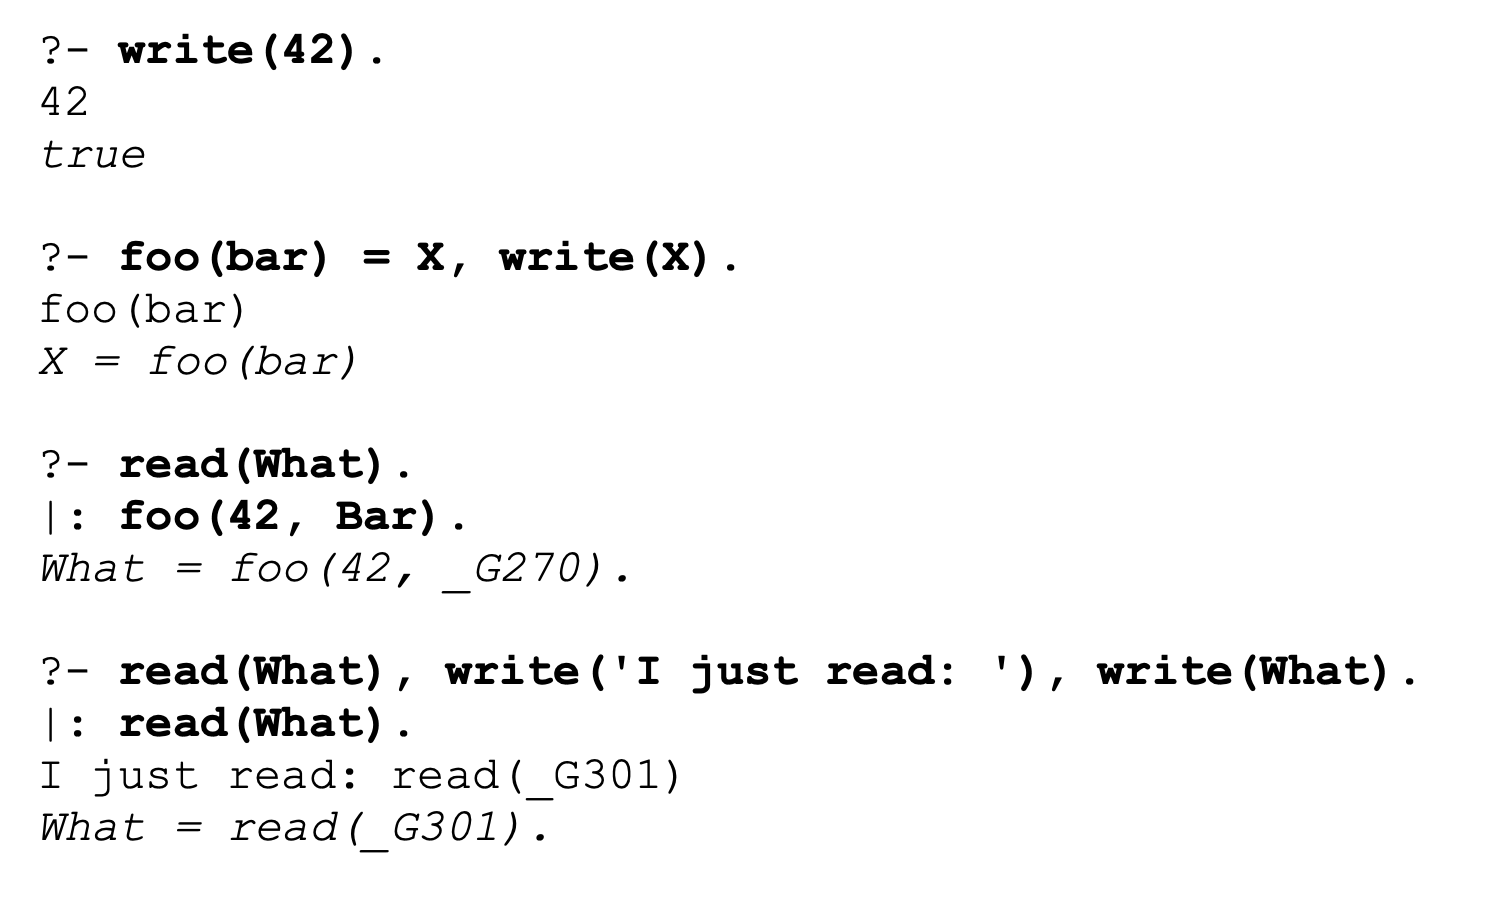
\includegraphics[width=0.75\textwidth]{esempi}
\end{center}
Analizziamo il terzo di questi che è già abbastanza complesso: 
read(What). praticamente cosa fa? Legge ed unifica con la variabile What. Quindi
quando passiamo foo(42, Bar), lui farà l'unificazione con questa. Cosa fa poi?
Praticamente Prolog ti scrive What = foo(42, \_G270). (Per i gamers, sì, anche
io ho pensato al G27).
\section{Open \& Close}
Sempre dalle slides vi riporto gli esempi:
\begin{center}
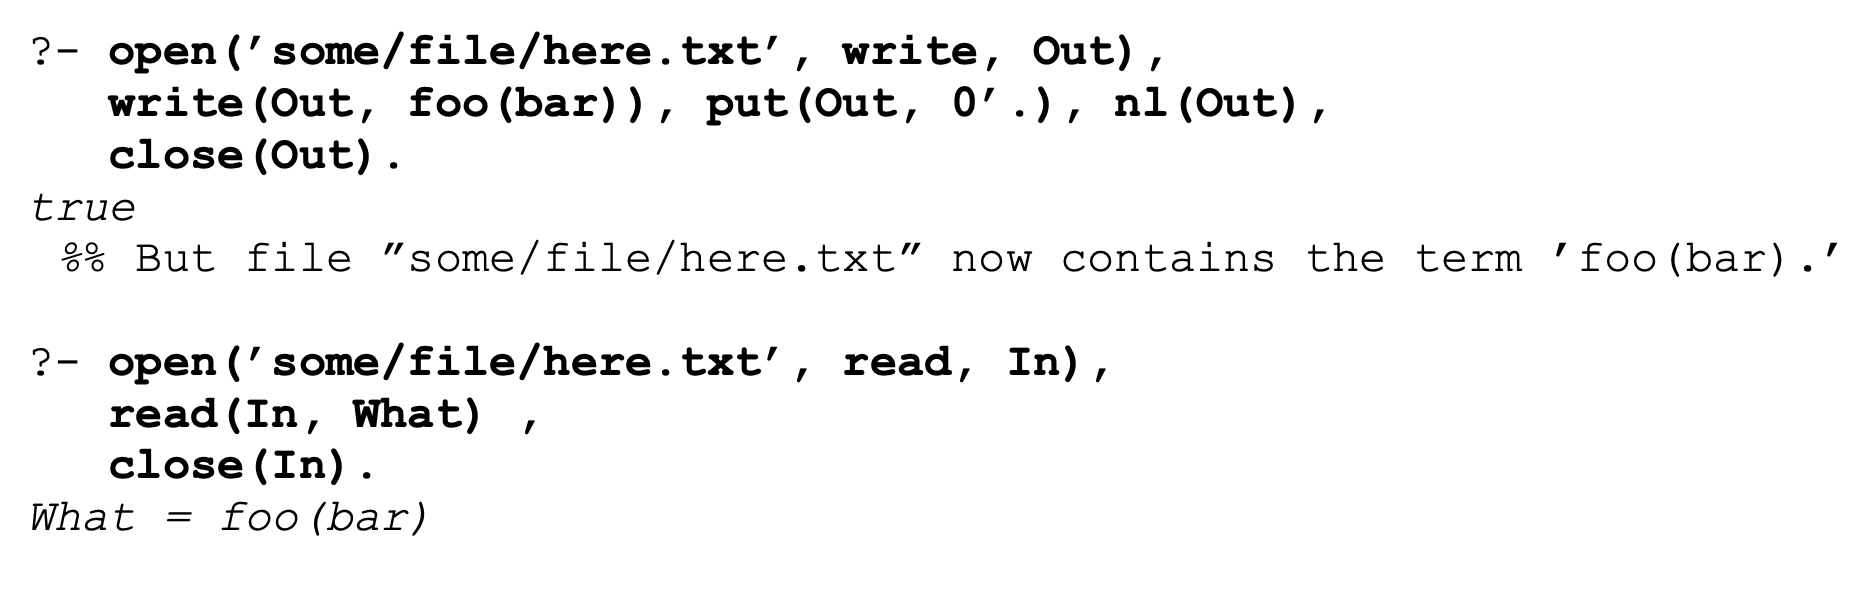
\includegraphics[width=0.75\textwidth]{openclose}
\end{center}
Come notiamo, l'open ha 3 argomenti che sono il percorso file, la modalità di
apertura e infine lo stream, che è rappresentato da Out. (Mi manca sinceramente
l'fopen di C/C++). \\ \\Sotto di fatto gli spariamo un write in Out con su scritto
foo(bar). Il put dopo? Niente, ci mette il punto dopo la funzione Prolog.
nl? Niente, fa il newline, il ritorno a capo, semplicemente. Inoltre
\begin{itemize}
	\item Prolog usa la notazione 0’c per rappresentare i caratteri come termini
	\item Put spara fuori SOLO un carattere, write una stringa.
	\item Il read di un file legge tutto quanto MA vedremo un altro parametro che
	aggiunge pure un limite di caratteri da leggere
\end{itemize}
\chapter{Interpreti in Prolog}
La domanda che spesso mi sono posto: Che schifo di linguaggio è un linguaggio in
cui per fare una somma devo soffrire ricorsivamente ogni singolo comando che 
scrivo? Risposta provvisoria: Bravissimi, ad un emerito *\textit{censura}*
\paragraph{Per l'appunto: }Prolog si presta ad utilizzi del tipo parsers o 
interpreti, ma come si può costruire un interprete che (non deterministicamente)
riconosca dei linguaggi regolari? Dalle slide spunta questo codice:
\begin{center}
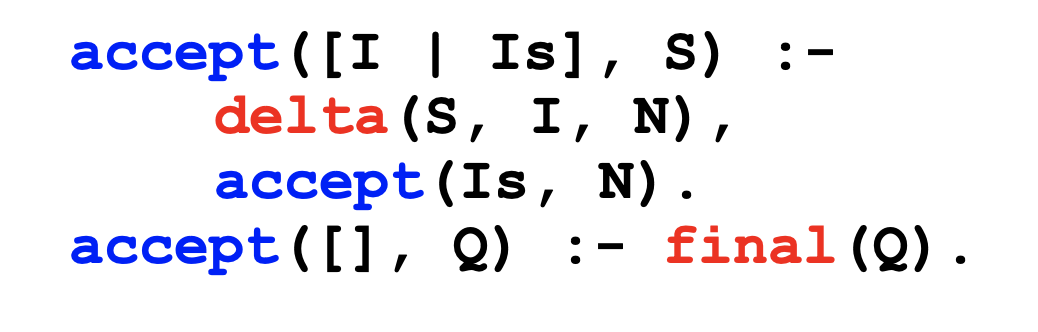
\includegraphics[width=0.75\textwidth]{accept}
\end{center}
Data una stringa, questo frammento ti dice se si accetta o no la suddetta. Come
ragiona? 
\begin{itemize}
	\item Se ho una transizione da S ad N con un simbolo i (delta indica le
	transizioni) allora accetta la stringa
\end{itemize}
E mi rendo conto che darti un codice senza contestualizzarlo sia un po' infame
da un certo punto di vista, perciò vediamo un automa che almeno è più 
comprensibile
\begin{center}
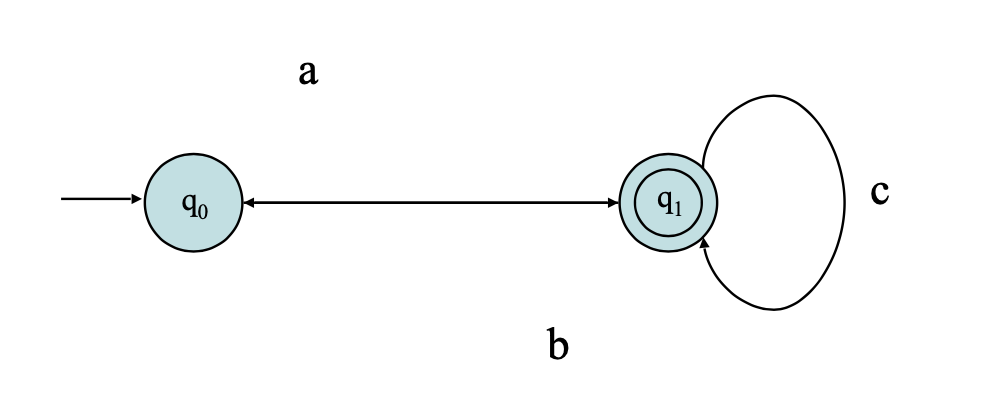
\includegraphics[width=0.75\textwidth]{autom}
\end{center}      
Come va a codificarsi questo automa?
\begin{lstlisting}[language=Prolog]
initial(q0). final(q1).

delta(q0, a, q1). 
delta(q1, b, q0). 
delta(q1, c, q1).
\end{lstlisting}
Per decidere se una certa sequenza di simboli è riconosciuta dall’automa 
possiamo costruire il seguente predicato:
\begin{center}
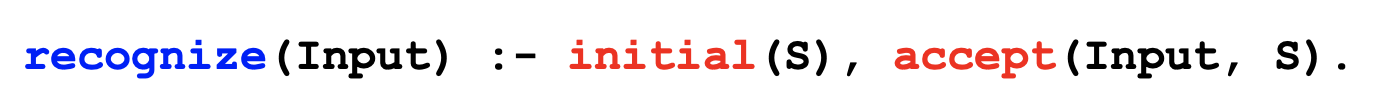
\includegraphics[width=0.75\textwidth]{reco}
\end{center}
\section{Interprete di un CFG}
\begin{center}
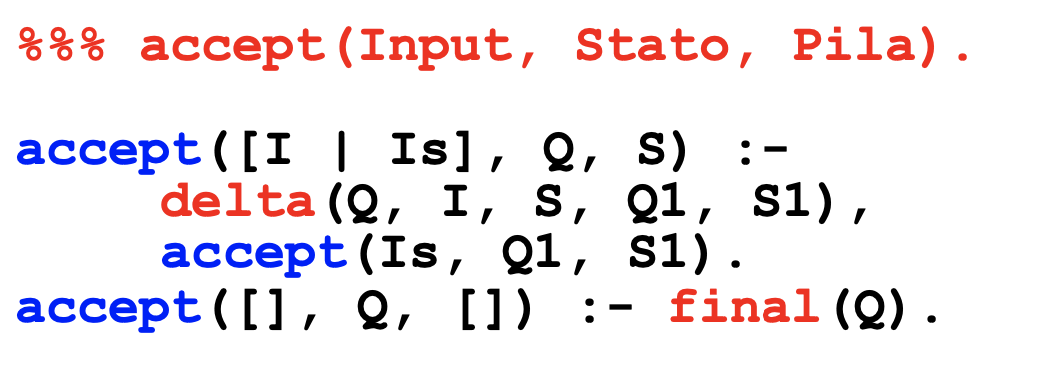
\includegraphics[width=0.75\textwidth]{acceptpila}
\end{center}
Considerando il linguaggio $L=\{wrw^{R}|w \in\{a,b,c\}^{n} \wedge n\geq0$.
Quello che accade è che l'automa verrà codificato così
\begin{center}
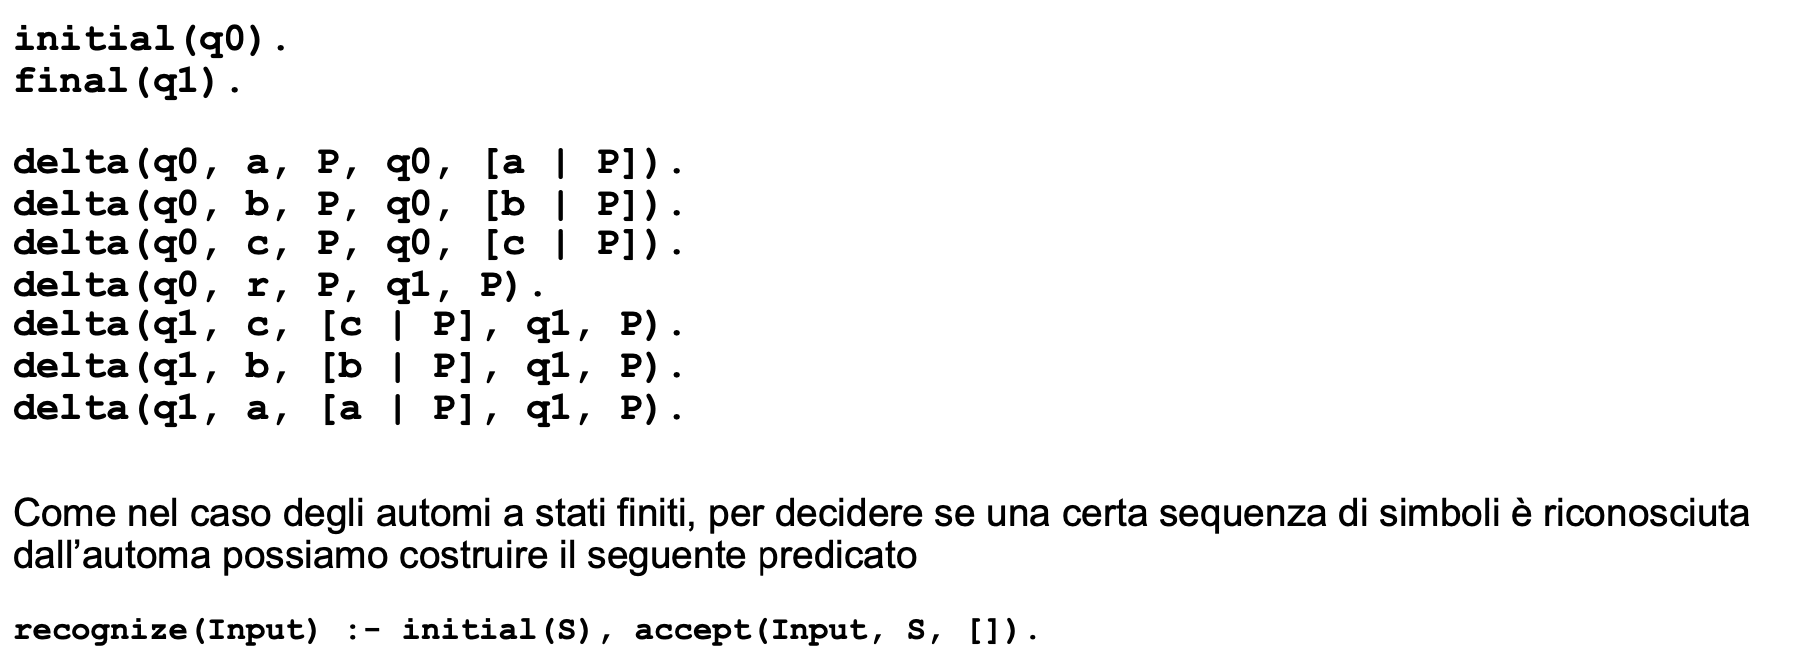
\includegraphics[width=0.75\textwidth]{codificaauto}
\end{center}
\section{Meta-Interpreti}
Il predicato call in pratica è il più semplice \textbf{meta-interprete},
chiaramente possiamo scrivere degli interpreti pi complessi e specializzati
se accettiamo di rappresentare i programmi con una sintassi leggermente 
diversa.
\paragraph{Ok, ma cosa ci possiamo fare? }Definiamo un predicato 
\begin{lstlisting}[language=Prolog]
solve(Goal :- solve(Goal, [])).
solve([], []).
solve([], [G | Goals]) :- solve(G, Goals). 
solve([A | B], Goals) :- append(B, Goals, BGoals),
solve(A, BGoals). 
solve(A, Goals) :- rule(A),
solve(Goals, []). 
solve(A, Goals) :- rule(A, B), 
solve(B, Goals).
\end{lstlisting}
\textbf{solve} diventa un meta-interprete per i predicati \textbf{rule}che
compongono il nostro sistema.
\paragraph{Ragionando per Incertezza invece}
\begin{lstlisting}[language=Prolog]
solve_cf(true, 1) :- !.
solve_cf((A, B), C) :- !, solve_cf(A, CA), 
solve_cf(B, CB),
minimum(CA, CB, C).
solve_cf(A, 1) :- builtin(A), 
!, 
call(A).
solve_cf(A, C) :- rule_cf(A, B, CR), 
solve_cf(B, CB), 
C is CR * CB.
\end{lstlisting}	
Devo mi sa rivedermi l'indentazione, spero sia corretta. 
Appena riesco sistemo questa cosa.
\chapter*{Conclusione di Prolog}
Prolog non è altro che un linguaggio in grado di esprimere problemi, conoscenze
e soluzioni in modo naturale (Eh.. 'na robba. naturalissimo guarda.). Lo stile
è lo stile \textbf{Dichiarativo}, il suo uso è efficace nella programmazione di 
sistemi deduttivi.\\ \\
Lo stile di programmazione del Prolog e le idee alla sua base sono i componenti 
principali di una serie di nozioni utili alla gestione di relazioni semantiche
su Web (RDF)
\chapter{Linguaggi Funzionali (SECONDO PARZIALE)}
Prima di parlare effettivamente di questo paradigma di programmazione, bisogna 
menzionare un argomento importante.
\section{Trasparenza referenziale}
Allora, con calma, è una proprietà, ed è valida per espressioni 
matematiche, e rende possibili le sostituzioni di espressioni con altre, basta 
che hai gli stessi valori. 
\paragraph{Eh.. Cioè? }Prendi f(x) + g(x), sono sostituibili con delle nuove
funzioni f e h Se e SOLO se effettivamente produciono gli stessi valori. (Si, 
oddio, più che funzioni, f e h scritte così sembrano variabili)
\subparagraph{Eeeee... Quindi?} Niente, per quanto riguarda LISP, ed i linguaggi
funzionali in generale, si ha questa trasparenza referenziale come "fondamento".
\paragraph{Lo stile }NON è più dichiarativo, qua è una funzione, una super mega 
giganteschissima funzione, più precisamente è una combinazione di tutte le mie 
varie funzioni. La composizione di funzioni è la chiave.
Quello che accade è che definiremo funzioni per poi andare ad usarle, 
tutto lì. Le regole delle funzioni vengono applicate.
\paragraph{Anche qui è tutto ricorsivo: }I cicli non ci sono, come non c'erano
in Prolog, gli assegnamenti si possono circa fare, ed è tutto di nuovo 
ricorsivo. Ah sì, per il resto tutto funzioni, tutto completamente a funzioni.
\chapter{LISP}
\textbf{LIS}T Processing, cioè elaborazione delle liste, nasce verso la fine 
degli anni 50 (Siamo solo nel 2019, not bad), successivamente poi LISP si è 
evoluto in altri sottoLinguaggi (Tipo le fork su GitHub) come Common LISP e 
Scheme, noi useremo Common LISP. 
\paragraph{L'ambiente }NON è compilato, o meglio, dovrebbe non esserlo, perchè
si ha un interprete tipo Prolog.
L'interprete \textbf{VALUTA TUTTO}, argomenti della funzione compresi. T U T T O.
Non metterò più di tanta roba, vi lascio giusto qualche esempio.
\begin{center}
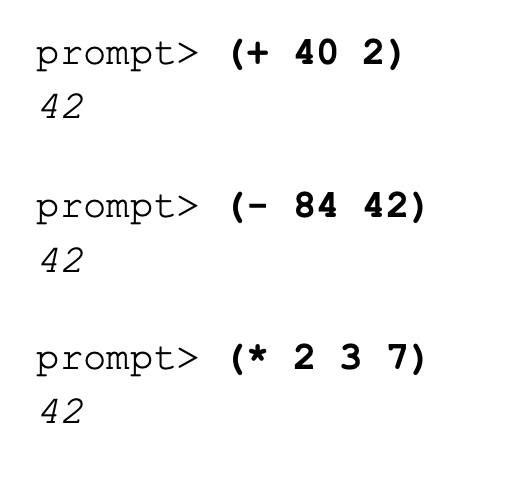
\includegraphics[width=0.75\textwidth]{10}
\end{center}
\begin{center}
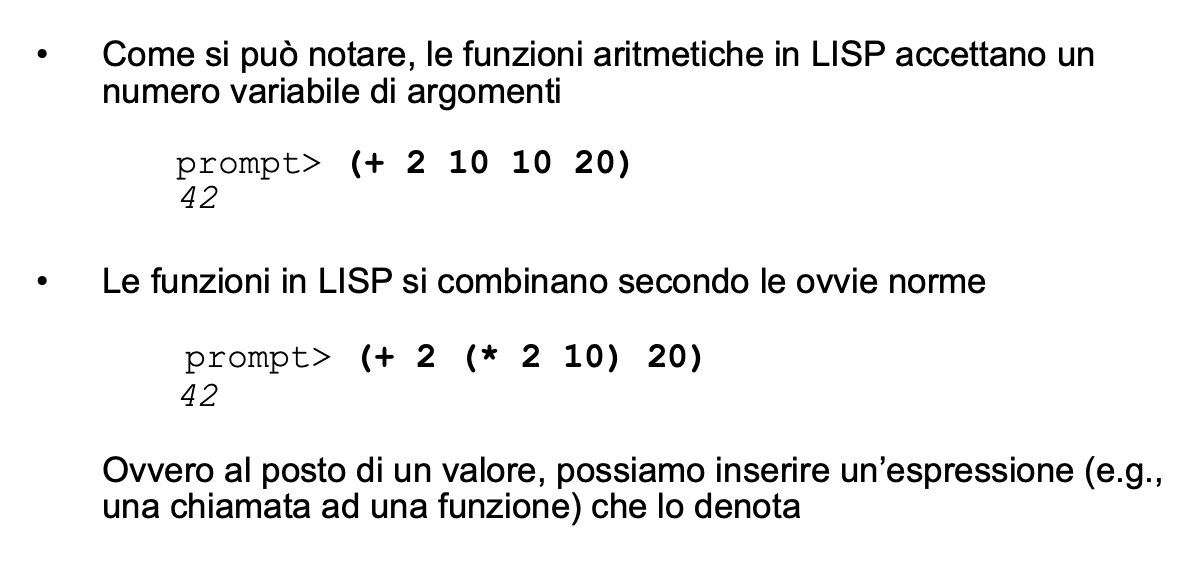
\includegraphics[width=0.75\textwidth]{11}
\end{center}
\section{Introduzione}
Di base LISP è composto di funzioni. Un esempio di funzione potrebbe
essere ad esempio
\begin{lstlisting}[language=LISP]
prompt> (+ 3 5)
8
\end{lstlisting}
Come già da qua si vede c'è una funzione definita tutta tra parentesi. Si apre 
con + (indica che funzione è) e poi gli argomenti della funzione che si considera.
Ora, c'è un detto famoso: \textbf{LISP è il miglior simulatore di parentesi}. 
Basti pensare che se voglio fare una somma dentro una somma mi vien fuori
\begin{lstlisting}[language=LISP]
prompt> (+ (+ 4 6) 5)
15
\end{lstlisting}
Immaginatevi cosa vien fuori tra poco.
Dalle slide vi riporto qualche esempio più preciso: 
\begin{center}
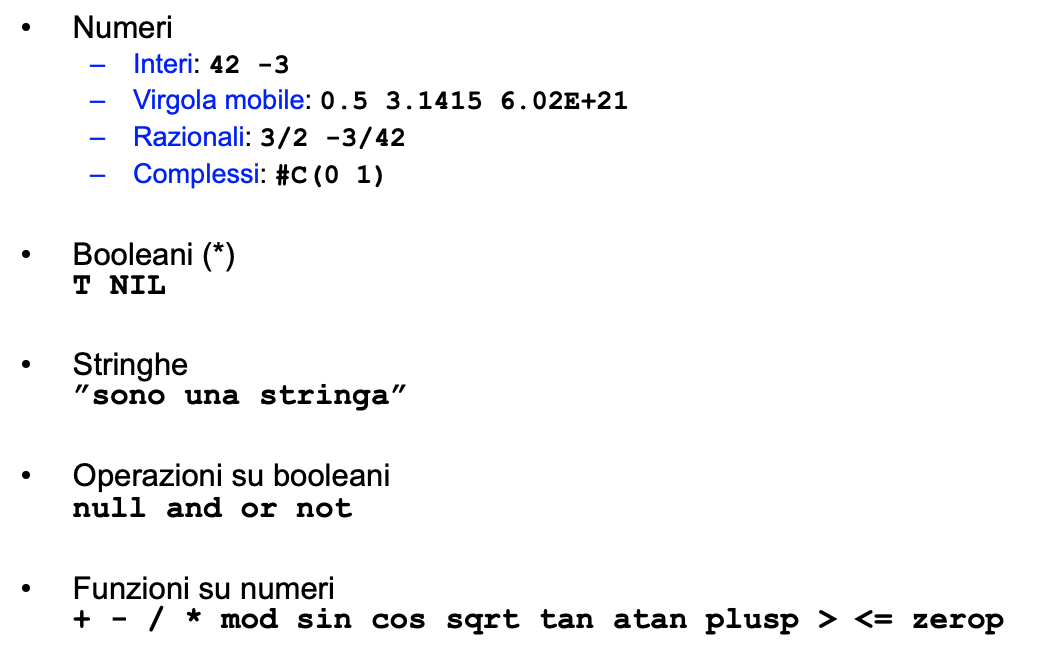
\includegraphics[width=0.75\textwidth]{12}
\end{center}
Inoltre bisogna anche mettersi nell'ottica che se Prolog funzionava tutto al 
contrario, invece LISP no, funziona in ordine da sinistra verso destra.
Anche qui non sto a insistere troppo, riporto diretto dalle slide.
\begin{center}
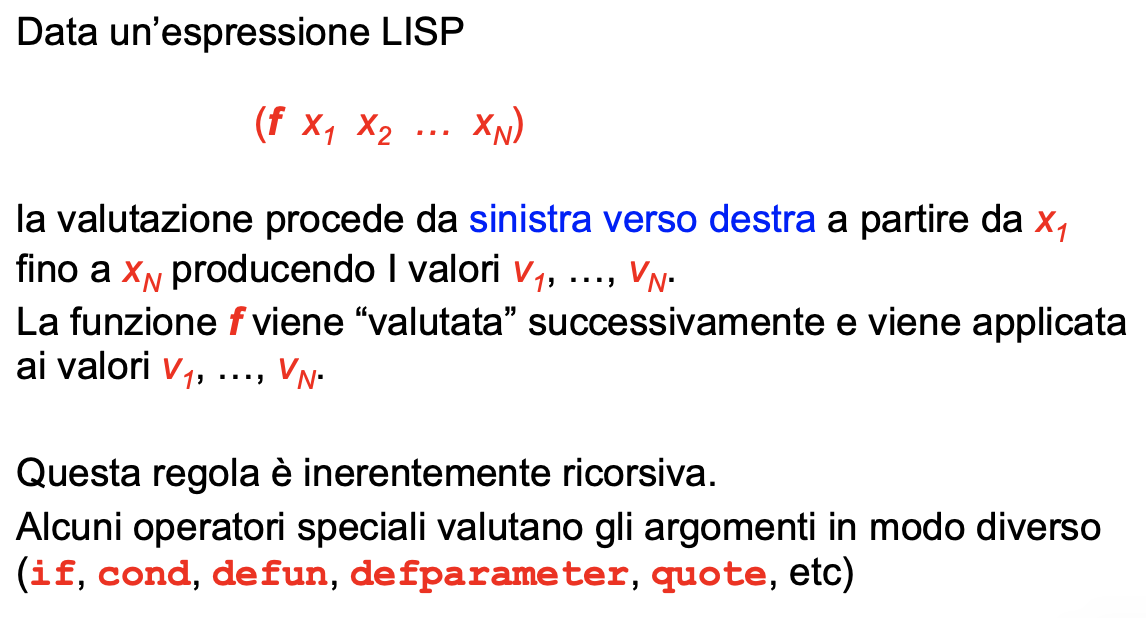
\includegraphics[width=0.75\textwidth]{13}
\end{center}
L'interprete realizza il suo parsing partendo da sinistra e procedendo 
ricorsivamente verso destra, easy, riconosce i simboli etc.
\paragraph{Osservazione: }$v_{1}$ è prodotto da $x_{1}$, nel senso che 
siccome l'interprete ragiona su ogni elemento delle parentesi
\subsection{Come definisco una funzione o una variabile}
Ci son due funzioni predefinite per questo scopo che sono \textbf{defparameter}
e \textbf{defun}, uno definisce un parametro, per ipotesi se avessi:
\begin{lstlisting}[language=LISP]
prompt> (defparameter x 15)
15
\end{lstlisting}
In java avremmo scritto
\begin{lstlisting}[language=Java]
x = 15;
\end{lstlisting}
(Mancherebbe il tipo per i dati ma.. Non c'è in questo caso). Ci sono diversi 
modi per fare gli assegnamenti, in questo caso si ha defparametere come base ma 
ne vedremo migliori più avanti.
Definiamo ora una ipotetica funzione: 
\begin{lstlisting}[language=LISP]
prompt> (defun quadrato(x) (* x x))
quadrato
\end{lstlisting}
E' come aver fatto in java
\begin{lstlisting}[language=Java]
public int quadrato(int x){
return x * x;
}
\end{lstlisting}
E' abbastanza intuitivo, una volta definite le nostre funzioni e costanti, 
possiamo poi utilizzarle ovviamente
\begin{lstlisting}[language=LISP]
prompt> (quadrato x)
1764
\end{lstlisting}
Qua si lavora con simboli, non stringhe, occhio a non confondersi su questa cosa.
\section{Funzioni $\lambda$ (Funzione anonima)}
In pratica si possono costruire delle funzioni che siano anonime, dette anche 
funzioni $\lambda$. 
In parole povere lambda è una funzione che però non ha un nome. 
\paragraph{A che serve?} Puoi direttamente applicarla a degli argomenti, tipo 
per dire
\begin{lstlisting}[language=LISP]
prompt> (lambda (x) (+ 2 x))
%In pratica aggiungo 2 ad x
prompt> ((lambda (x) (+ 2 x))40)
\end{lstlisting}
Ogni volta si deve star lì a ridefinirsela insomma, capiamo già da qui che ha 
più senso (in base alla riusabilità) definirsi di pacco una funzione e stop.
Per ora lasciamole un po' da parte, più tardi ci serviranno di più. 
Ora, proviamo a definirci una funzione del tipo valore\_assoluto.
A cosa è uguale? 
\[
valore\_Assoluto = \begin{cases}
x ~ se ~ x > 0 \\
0 ~ se ~ x = 0 \\
-x ~ se ~ x < 0
\end{cases}
\]	
Bene, questo da un punto di vista prettamente matematico, ma invece come sarebbe
dal punto di vista più programmativo? In questo caso c'è il \textbf{cond}. 
E' una funzione che associa semplicemente elemeti tra loro.
\begin{lstlisting}[language=LISP]
(cond (x a) (y b))
\end{lstlisting}
In pratica associa x con a e y con b, con x, a, y, b che sono delle espressioni.
\begin{lstlisting}[language=LISP]
(defun valore-assoluto (x) 
(cond ((> x 0) x)
((= x 0) 0)
((< x 0) (- x))))
\end{lstlisting}
Da qui abbiamo un esempio carino anche di indentazione del codice. 
Non c'è molto da dire su < > e =, sono delle booleane che o danno True o False.
Se ci son le booleane c'è anche l'\textbf{if}, che funziona come una qualsiasi 
funzione booleana 
\begin{lstlisting}[language=LISP]
defun(maggiore_di_zero (x))
(if (> x 0) T) 
\end{lstlisting}
In pratica ti spara True se lo è, come si osserva non c'è l'else, perchè va in
successione all'altra espressione.
Proviamo a definire una funzione ricorsiva, il fattoriale.
\begin{lstlisting}[language=LISP]
(defun fattoriale (n)
(if (= n 0) 1
(* n (fattoriale (- n 1)))))
\end{lstlisting}
Tradotto, se n è 0 allora dammi 1 altrimenti dammi il prodotto di n con il 
fattoriale di n-1. Manca l'else, ma da qua si capisce che vien fatto in sequenza.
\paragraph{E' tutto ricorsivo: }Come in Prolog tutto va ricorsivamente, PERCIO' 
sarà possibile in qualche modo tentare di simulare un'iterazione.
\begin{lstlisting}[language = LISP]
(defun fatt-ciclo (n acc) 
(if (= n 0)
acc
(fatt-ciclo (- n 1) (* n acc))))

(defun fattoriale (n) 
(fatt-ciclo n 1))
\end{lstlisting}
In pratica gli chiedo, è n = 0? restituisco l'accumulatore, quindi questo si 
incrementerà costantemente, infatti dopo si ha il fattoriale di n - 1 che 
va a prendere l'accumulatore e lo moltiplica per n.
Sotto infatti abbiamo che il fattoriale di n è il risultato di questa iterazione.
\paragraph{Questa struttura si chiama ricorsione in coda: }Ovvero la ricorsione 
è \textbf{L'ultima} operazione che eseguo. Per intenderci, la funzione di fibbonacci
NON è eseguibile così, perchè funziona con due ricorsioni attive. 
\section*{Ricorsione}
Dato un insieme di funzioni mutualmente ricorsive, questo può rappresentare una 
macchina di Turing, pertanto i linguaggi funzionali puri (senza assegnamenti e
salti) sono \textbf{Turing Completi}
\section{Strutture per i dati e funzioni}
Ipotizziamo di dover costruire una libreria per fare dei calcoli su numeri 
razionali. Di cosa ci sarà bisogno? Innanzitutto si deve assumere di avere a 
disposizione una funzione che costruisce una \textit{Reppresentazione} di un 
numero razionale:
\paragraph{Banalmente: } (\textbf{crea-razionale n d}) $\implies <razionale \frac{n}{d}$>
Ora però ci servono due funzioni per definirci il numeratore ed il denominatore
\begin{itemize}
	\item numer
	\item denom
\end{itemize}
A questo punto è easy crearsi una libreria (Sieh, è già tanto se so scriverti 
una somma, sicurissimo so farti la libreria guarda), e vien fuori una roba del 
genere:
\begin{center}
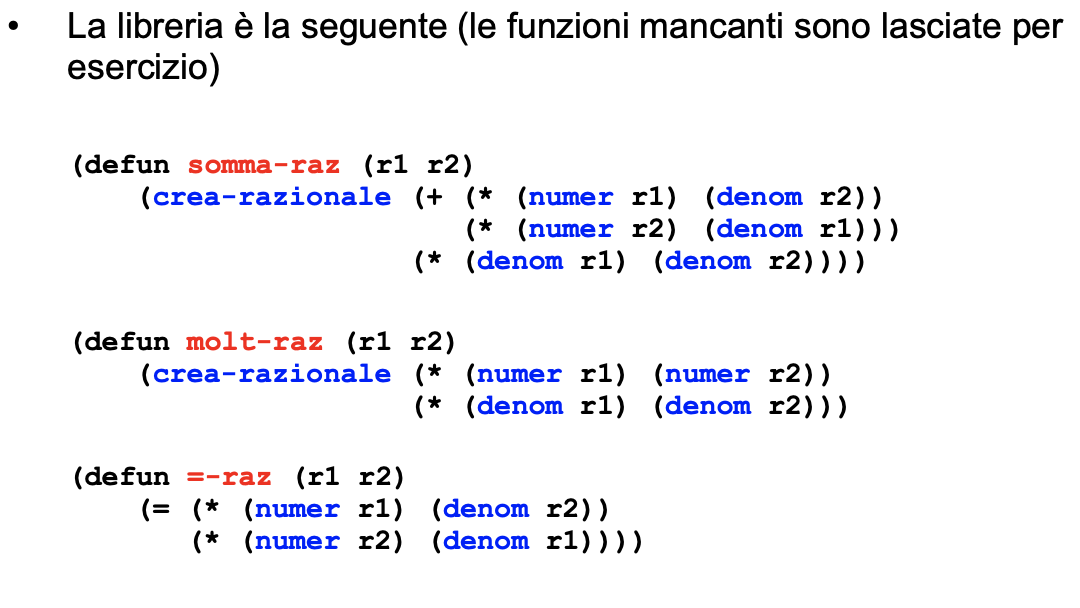
\includegraphics[width=0.75\textwidth]{14}
\end{center}
\section{Cons-Cells e funzione CONS}
Una struttura essenziale è la cons-cell, cioè una coppia di puntatori a due 
elementi.
Sono create dalla funzione \textbf{cons} che praticamente alloca della memoria 
(E' tipo malloc di C oppure un new in Java) 
\begin{center}
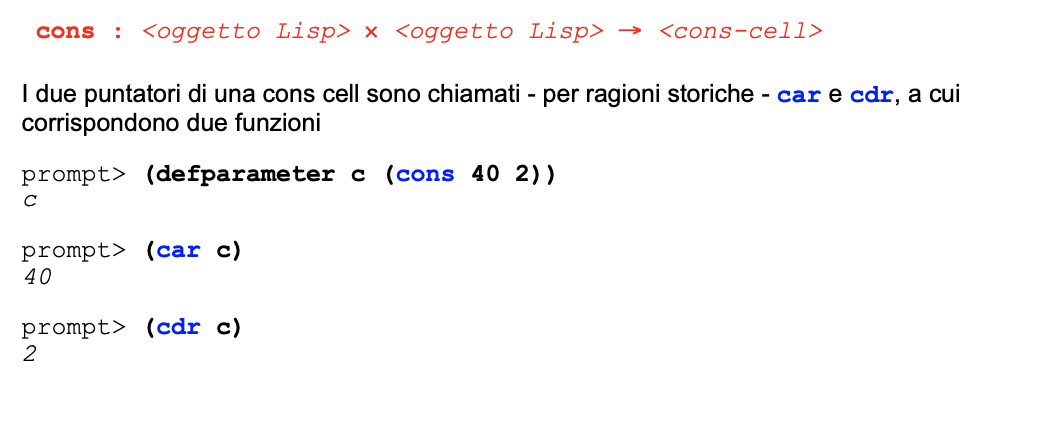
\includegraphics[width=0.75\textwidth]{15}
\end{center}
\section{Rappresentazione dei numeri razionali}
In pratica tu hai la tua primitica cons, e hai delle funzioni che sono
\begin{itemize}
	\item Crea-razionale
	\item numer
	\item denom
\end{itemize}
che vengono schematizzate così: 
\begin{center}
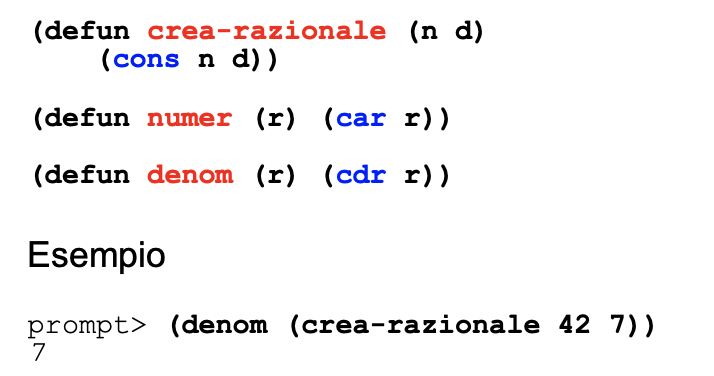
\includegraphics[width=0.75\textwidth]{16}
\end{center}
Visto che si è menzionato qualcosa di più grafico, proviamo a dare un che di 
informativo a ciò che abbiam detto. Come detto primo quello che fa la conf è:
\begin{itemize}
	\item Generare una coppia di puntatori
\end{itemize}
Si possono ottenere dei veri e propri grafi che sono in una notazione box and 
pointer, come in questa illustrazione:
\begin{center}
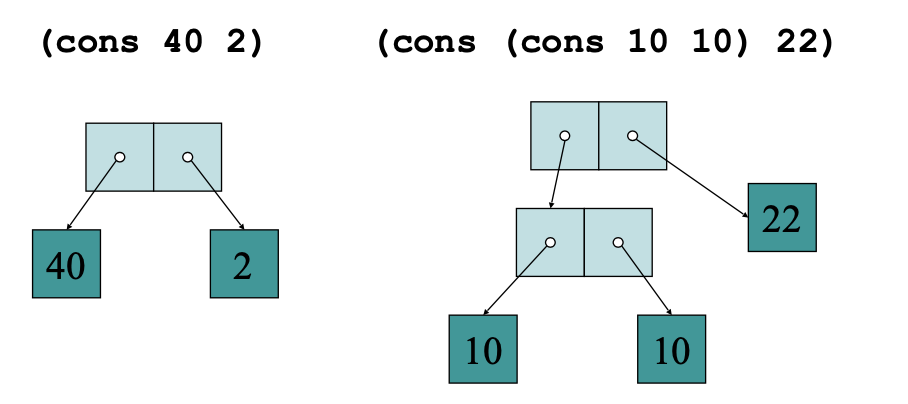
\includegraphics[width=0.75\textwidth]{17}
\end{center}
\paragraph{Precisazione: }Quando disegnate questi grafi aspettate un attimo prima
di scrivere i numerelli dentro i quadratini.
Ok e se voglio fare un puntatore che punta ad un solo elemento? Niente, invece 
di metterci un valore gli do NIL che sarebbe un puntatore a.. niente. Nel senso
lista vuota, ma il senso è quello. 
\paragraph{Come si comporta LISP quando gli diamo un cons}?\\
Esplode, perchè ci odia palesemente :)\\
Scherzi a parte, si ha una notazione "dotted-pair" che praticamente è una coppia
separata da un punto, in cui gli spazi son significativi. (NIL . T), che è il 
corrispettivo di una funzione (cons NIL T).
\subparagraph{Lamentela mia:} Sarò fastidioso, ma mi urta il sistema nervoso 
"NIL", ma non potevan chiamarlo NULL come tutte le persone normali? No? Vabbeh.
Ora sono offeso :c
\subparagraph{Edit: }A quanto pare più avanti si vedrà che null è una funzione,
e quindi.. Han dato il nome di un valore ad una funzione, giusto per confondermi
meglio	
\paragraph{Occhio a una cosa:} Se io pongo (cons 42 nil) ottengo una lista avente
solo un numero che è 42, invece se fosse (cons nil 42) non è una lista, è una 
cosa un po' diversa, \textbf{altra cosa importante: }Se notiamo, quello che 
accade è che facendo (cons a nil), si ottiene una lista, perciò se al posto di 
nil ci fosse un'altra lista tipo (cons a (cons a nil)), in pratica aggiungi una
lista a dentro una lista quindi hai una lista con dentro una lista, mentre 
se vuoi aggiungere solo l'elemento devi usare (cons a (cons nil a)), che 
concatena alla prima lista il nuovo carattere semplicemente. 
\section{Esempi sulle liste}
\paragraph{Esempio 1}
\begin{center}
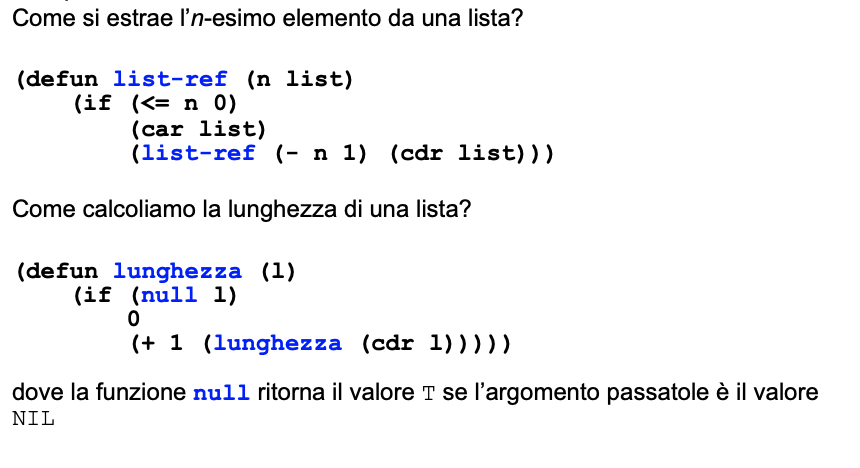
\includegraphics[width=0.75\textwidth]{18}
\end{center}
In pratica quello che accade è che: \\
La funzione list-ref si definisce con il nome nth (Per via di Common Lisp),
mentre invece la funzione cdr ritorna il resto di una lista, inteso come "tutti"
gli altri elementi meno la testa, quindi si ha in common lisp il "rest".
\paragraph{}
Ora, la funzione car torna invece il primo elemento della lista, la testa, e 
qua si segna con first infatti, al fine di evitarci le combinazioni standard si 
ha che :
\begin{lstlisting}[language=LISP]
(car (cdr L))
(car (cdr (cdr L))
(car (cdr (cdr (cdr L)))) 
...	
\end{lstlisting}
Common lisp ha in libreria le funzioni second, third, fourth fino a tenth, cioè
fino al decimo elemento.. credo.. della lista(?) A logica è quello.     
\paragraph{Esempio 2: Concatenazione delle liste}
Anche qui c'è l'append, che letteralmente prende due parametri che sarebbero due 
liste (pure la lista vuota) e quel che fa è concatenarle, se però una delle
due liste è vuota, ti spara quell'altra e basta.
\section{Espressioni simboliche}
Se in prolog avevamo le clausole di horn qui ci sono fondamentalmente
\begin{itemize}
	\item Numeri
	\item Simboli
	\item Stringhe
	\item Cons-cells
	\item Oggetti di base di LISP
\end{itemize}
CIoè fondamentalmente pure qua ci sono espressioni simboliche (sexp's) che sono
a tutti gli effetti costituite dalle cons-cells
\begin{itemize}
	\item Dato che programmi e sexp’s in Lisp sono equivalenti, possiamo dare
	le seguenti regole di valutazione (ed implementarle nella funzione eval!)
\end{itemize}
Data una sexp: 
\begin{center}
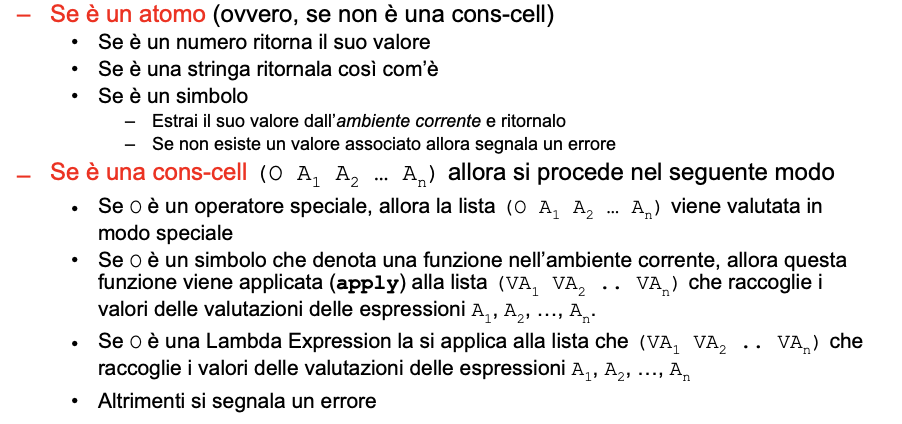
\includegraphics[width=0.75\textwidth]{19}
\end{center}
Ora vi riporto gli esempi dalle slide di funzioni ricorsive:
\begin{center}
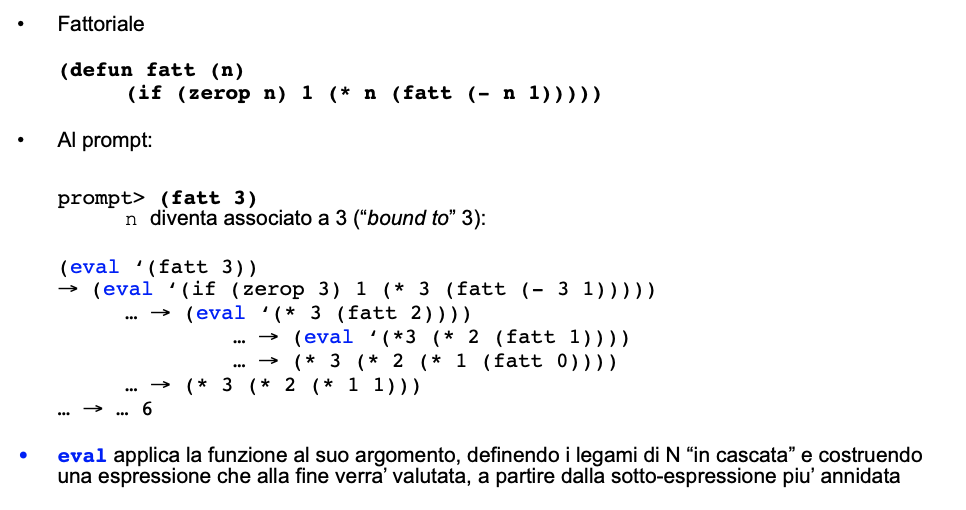
\includegraphics[width=0.75\textwidth]{20}
\end{center}
Il concetto è che la forma ricorsiva delle liste si presta bene alla programmazione
ricorsiva.. Cioè ovviamente direi.
Come?
\begin{itemize}
	\item Scrivo il valore della funzione nel caso base
	\item Ricorsivamente mi devo ridurre al caso base operando su un argomento
	ridotto, minore, decrementato. FINCHE' non sarà 0 o il caso base.
\end{itemize}
\section{Operatori di uguaglianza}
Si hanno due differenti operatori per verificare l'uguaglianza tra due oggetti:
\begin{itemize}
	\item eql
	\item equal
\end{itemize}
\subsection{Eql}
E' applicato a simboli e numeri interi e puntatori. In pratica ti dice
se due valori sono uguali, tipo (eql 'a 'a):
\paragraph{}In pratica gli chiedi: è la stringa "a" uguale alla stringa "a"? 
Ma potrebbe pure esserci un valore numerico
\subsection{Equal} \textbf{equal} è esattamente come \textbf{eql} ma va 
a scavare in profondità alle liste, nel senso che applica ricorsivamente a tutte 
le sottoliste presenti l'eql. 
\subparagraph{Esempio: }prendi la lista (((((a))))), in pratica hai una serie di 
sottoliste che ricorsivamente devi andarti a calcolare, equal fa anche questo, 
quindi è più figo, potente.
\section{Il vantaggio del paradigma funzionale}
Una volta capito cos'è il quote, la lista possiamo finalmente dare un senso 
all'esistenza di questo tipo di paradigma. 
\paragraph{Per esempio: }prendete la lista 
\begin{lstlisting}[language=LISP]
(defparameter pari (list 2 4 6 8 10))
\end{lstlisting}
E supponismo ora che per ipotesi volessimo moltiplicare tutti gli 
elementi di questa lista per un determinato valore (In pratica prodott di un 
vettore per $\kappa$)
\begin{lstlisting}[language=LISP]
(defun scala-lista (l fattore) 
	(if (null l)
		nil
		(cons (* fattore (car l))
				(scala-lista (cdr l) fattore))))	
\end{lstlisting}
Notare che questa funzione che certamente mi ricordo già a memoria.. Vero? usa
una ripetizione di append, l'operazione fa questa funzione si può astrarre se 
andiamo ad astrarre il concetto di valore funzionale.
\paragraph{Cioè? }L’astrazione “ \color{red} applica la funzione f a tutti gli 
elementi della
lista L e ritorna una lista dei valori”\color{black} è nota come “map”; in
Common Lisp la 
funzione mapcar svolge questo compito.
\paragraph{Mapcar} è una funzione predefinita ma è riscrivibile come:
\begin{lstlisting}[language=LISP]
(defun mapcar* (funzione lista)
       (if (null lista)
			nil
			(cons (funcall funzione (car lista))
					(mapcar* funzione (cdr lista)))))	
\end{lstlisting}
In cui mapcar* è usato per evitare errori in CommonLisp, e si noti inoltre anche
\textbf{funcall} che invece chiama la funzione prendendo un certo argomento.
\paragraph{Qua ci sono alcuni esempi presi dalle slide}
\begin{center}
	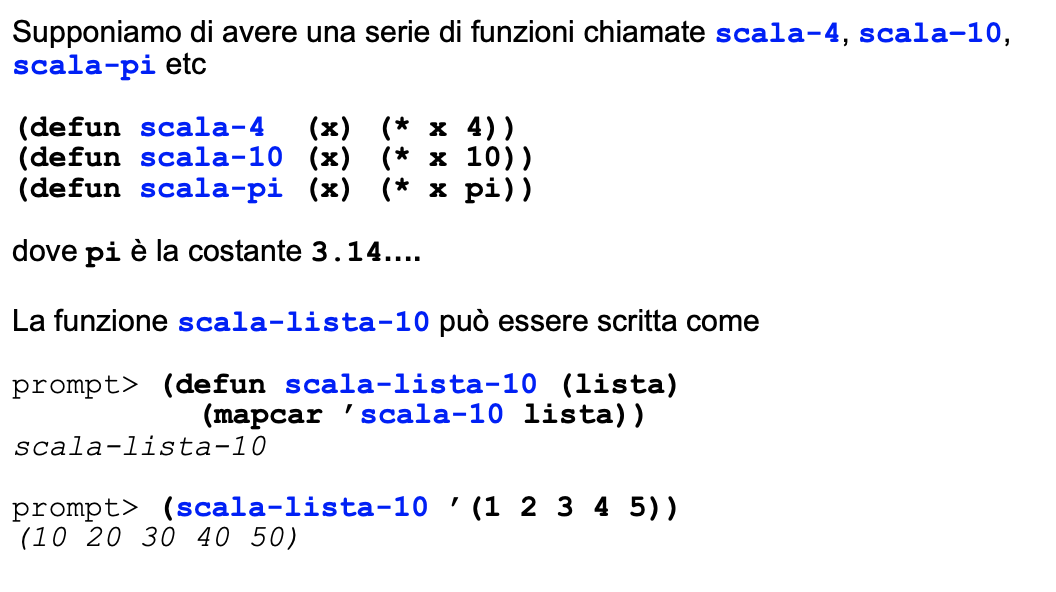
\includegraphics[width=0.75\textwidth]{21}
\end{center}
\section{$\lambda$-Funzioni}
Avevo voglia di scrivere $\lambda$ come simbolo a caso, ma quando si useranno 
queste funzioni si usa \textbf{lambda}, che serve per indicare delle funzioni 
anonime, praticamente costruisce delle funzioni quando ce n'è bisogno.
\paragraph{Cioè? }In LISP è possibile definire queste funzioni in modo che ti 
definisci unas funzione solo quando ti serve. Una volta creata, la usi, ma appena
finito di usarla *puf*, morta, schiattata, defunta, REST IN PEACE BOI. Consente
sicuramente di ottimizzarsi meglio la memoria
\paragraph{Esempi: }
\begin{center}
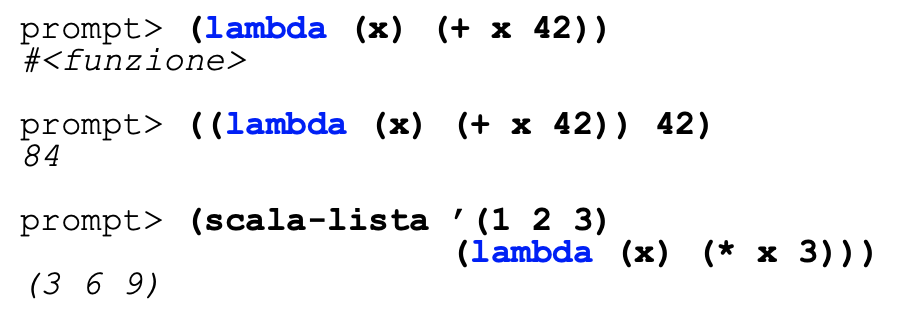
\includegraphics[width=0.75\textwidth]{22}
\end{center}
In pratica il concetto è che con il lambda puoi generare delle funzioni che 
si basano su quest'ultima: Per intenderci se voglio fare una funzione che si 
chiama "IncrementaDi" con x come parametro, la \textbf{lambda} praticamente 
si può strutturare con un (+ x y), perciò si definisce una funzione:\\
(defun incrementa-x (x) 
	(lambda (y) (+ x y)))\\
Se per ipotesi ora si volesse fare una funzione che ti somma 5 diventerebbe
(defun incrementa-5 (x) (incrementa-x 5))
\section{Let}
Prendiamo una funzione di questo tipo:
\[
	f(x, y) = x(1+xy)^{2}+y(1-y)+(1-y)(1+xy)
\]	
In pratica tu usando lambda puoi costruirti tutti i valori intermedi, e quel che
accade è che la funzione vien chiamata con due valori che saranno i valori 
intermedi da usare:
\begin{lstlisting}[language=LISP]
(defun f (x y)
      ((lambda (a b)
          (+ (* x (quadrato a))
             (* y b)
             (* a b)))
(+ 1 (* x y))
(- 1 y)))	
\end{lstlisting}
Questo tipo di chiamate a funzioni anonime è così utile da essere stato ri-codificato
con un nuovo operatore speciale: \textbf{let}
La funzione riportata qua sopra diventerebbe: 
\begin{lstlisting}[language=LISP]
(defun f (x y)
      (let ((a (+ 1 (* x y)))
		(b (- 1 y))
            )
         (+ (* x (quadrato a))
            (* y b)
            (* a b))))
\end{lstlisting}
Ovvero, l’operatore let ci permette di introdurre dei nuovi nomi (variabili) 
locali da poter riutilizzare all’interno di una procedura; la sua sintassi è la 
seguente.
\section{Funzioni di un ordine superiore}
Si intende ordine di una funzione quello che consiste nel prendere una funzione
e usarla come argomento di un'altra ma potrebbero essere anche di più. Il fatto che possiamo
implementare queste funzioni è fondamento del paradigma funzionale. Per ora
si è visto il \textbf{mapcar} ma ce ne sono altre tipo:
\begin{itemize}
	\item compose
	\item fold (o reduce)
	\item complement
	\item filter (variante di remove e delete)
\end{itemize}
\subsection{Compose}
E' l'equivalente della composizione di funzioni in matematica. La sua semantica è:
date due funzioni (di un unico argomento) f e g, mi deve tornare f di g(x), qui
ci torna di nuovo utile il \textbf{lambda}
\begin{lstlisting}[language=LISP]
(defun compose (f g)
   (lambda (x)
		(funcall f (funcall g x)))) 

prompt>	(funcall (compose 'first 'rest)
					'(1 2 3 4 5))
2
\end{lstlisting} 
Se per dire volessimo fare il fattoriale del 
\subsection{Filter}
E' un filtro, quindi rimuove tutti gli elementi che non rispettano una condizione.
Nel senso all'atto pratico è, prendo un elemento, SE quell'elemento non ha una
determinata caratteristica, non considero l'elemento. Praticamente è uno switch.
\begin{lstlisting}[language=LISP]
      (cond ((null lista) nil)
            ((funcall predicato (car lista))
             (cons (car lista)
                   (filter predicato (cdr lista)))
            (T (filter predicato (cdr lista)))))	
\end{lstlisting}
\subsection{Accumula}
Detta anche fold o reduce, praticamente progressivamente ha un valore che si
accumula in base al risultato ottenuto su ogni elemento della lista. Esempio:
La sommatoria di una lista, o la produttoria.
\begin{lstlisting}[language=LISP]
(defun accumula (f iniziale lista)
   	(if (null lista)
		iniziale
		(funcall f (car lista)
        		 (accumula f iniziale (cdr lista)))))
\end{lstlisting}
\chapter{Le Keywords}
I parametri invece di essere scritti in ordine possono essere anche associati
a dei nomi, delle keywords. Molte funzioni LISP hanno già questo di comportamento.
Tipo io prendo una lista (1 2 3 4 5 6 7 8 9 10) e posso dire che :start sia 3
e :end sia 10, quindi non mi serve averceli più in ordine. Se ad una 
funzione voglio dire che ciò che le arriva è una keyword devo usare \&key che
(defun make-point (\&key x y))\\
(list x y)\\
Quando noi lo richiamiamo possiamo chiamarla con: (make-point :y 5 :x 6), 
andrà ad assegnare ad x 6 e y 5 malgrado l'ordine sia invertito.

\chapter{Input/Output in Common LISP}
Come in ogni linguaggio anche qui ci sono funzioni che permettano di scrivere
in output e ricevere in input dati. E queste funzioni sono READ e PRINT.
Oltre all'input output su schermo posson pure prendere file.
\section{Read}
La Read semplicemente acquisisce e legge valori, è un input di oggetti LISP, 
in cui per oggetto si intende una lista, un valore, un carattere, tutto. 
\section{Output}
Ovviamente è bene avere metodi per stampare tipo con la write in Prolog, e 
Common Lisp ci mette a disposizione la funzione \textbf{FORMAT} (Avete 
presente fprintf in c? Ecco quello è il concetto). Va detto che è complessa
la \textbf{FORMAT}, prendiamo ad esempio qualcosa del tipo: 
\begin{lstlisting}[language=LISP]
prompt> (format t "il fattoriale di ~D e' ~D~%" 3 (fact 3))
il fattoriale di 3 e' 6
NIL
\end{lstlisting}
Le direttive in una stringa da formattare sono introdotte da \~, vediamone alcune
\begin{itemize}
	\item \~D stampa numeri interi
	\item \~\% ritorna a capo
	\item \~S stampa un oggetto Lisp secondo la sua sintassi standard
	\item \~A stampa invece un oggetto secondo una sintassi piacevole.. Che non
	so cosa voglia dire, ma oh, le cose piacevoli sono belle.
\end{itemize}
\section{Streams in CommonLisp}
Allora, ci son 3 tipi di stream, uno standard input, uno output, e uno error, che 
è più o meno come in java (syserr, sysout, sysin), inoltre le funzioni \textbf{Read,
print, e Format} accettano un numero variabile di argomenti, e uno di questi 
stream (di \textbf{output} per format e print e \textbf{input} per read).
\subsection{Manipolazione dei file}
Vi avviso, non è così semplice, perchè ci son diversi passaggi (è come in Java
più o meno, il funzionamento è lo stesso), non andremo in profondità su come si
gestiscono file di testo in LISP \underline{\underline{\textbf{MA}}}.
\paragraph{Di base:} per aprire un file si deve usare "\textbf{with-open-file}",
la sintassi precisa è la seguente: 
\begin{lstlisting}[language=LISP]
(with-open-file (<var> <file> :direction :input) <codice>)

(with-open-file (<var> <file> :direction :output) <codice>)
\end{lstlisting}
La variabile <var> è il nome dello stream, o meglio si associa allo stream aperto
sul file e può venire usata all'interno di <codice> cioè del segmento di codice
che andiamo a considerare. Tutto questo è \textbf{dentro} una funzione.
\paragraph{with-open-file} è una figata perchè si preoccupa di chiudere sempre e 
comunque lo stream associato a <var>, anche se ci sono errori.
\begin{lstlisting}[language=LISP]
(with-open-file (out "foo.lisp" 
					 :direction :output
					 :if-exists :supersede
					 :if-does-not-exist :create) 
	(mapcar (lambda (e)
			(format out "~S" e))
		'((1 . A) (2 . B) (42 . QD) (3 . D))))
\end{lstlisting}
Come già detto lo stream si chiude con l'ultima parentesi, ora apriamo lo stesso
stream ma in formato di input
\begin{lstlisting}[language=LISP]
(with-open-file (in "foo.lisp" 
			:direction :input
			:if-does-not-exist :error) 
	(read-list-from in))
\end{lstlisting}
In pratica in questo caso andiamo a vedere se un file c'è, se c'è appost, possiamo
modificarlo, altrimenti ritorniamo che c'è stato un errore.
\begin{lstlisting}[language=LISP]
(defun read-list-from (input-stream)
	(let ((e (read input-stream nil 'eof)))
		(unless (eq e 'eof)
			(cons e (read-list-from input-stream)))))
\end{lstlisting}
La cosa importante è il simbolo 'eof che indica per l'appunto l'end of file, 
ed in questo caso precisamente quello che stiamo dicendo è che quando arriviamo
alla fine deve uscire.
\section{Interazione con l'ambiente LISP}
Quando si parla di lisp, lavoriamo a linea di comando, ciò che fa quest'ultima
sono 3 operazioni fondamentali
\begin{enumerate}
	\item Leggere i comandi (\textbf{Read})
	\item Valuta con l'\textbf{eval} finchè non trova il risultato della valutazione
	\item Stampa il risultato della valutazione
\end{enumerate}
E tutto questo è praticamente un ciclo while(\textbf{true}), all'infinito. Ma
come funziona più precisamente questo loop? Come posso implementarlo in lisp?
La parte che segue è un po' più cicciosa di quella che abbiam visto finora, 
ci saranno un po' più cose da tenere a mente. 
\section{Apply ed Eval}
Dato che i programmi in lisp e sexp's sono equivalenti si può dare le seguenti 
regole di valutazione (ed implementare l'eval), questa roba servirà per il 
progetto.
\begin{itemize}
	\item Se è un atomo: cioè se non è una cons-cell
	\begin{itemize}
		\item Se è un numero ritorna il valore
		\item Se è una stringa la ritorna così come è
		\item Se è un simbolo
		\begin{enumerate}
			\item Estra il suo valore dell'ambiente corrente e lo ritorna
			\item Se non esiste un valore associato allora segnala un errore
		\end{enumerate}
	\end{itemize}
	\item Se è una cons-cell ($O A_{1}, A_{2}, A_{3}, ..., A_{N}$)
	\begin{itemize}
		\item Se O è un operatore speciale allora la suddetta lista vien valutata
		in modo speciale
		\item Se invece fosse un simbolo che denota una funzione allora viene 
		applicata (con l'\textbf{apply}) una lista ($VA_{1}, VA_{2}, ..., VA_{N}$)
		che praticamente raccoglie i valori delle valutazioni delle espressioni
		$A_{1}, A_{2}, A_{3}, ..., A_{N}$
		\item Se invece fosse una lambda expression la si applica alla lista 
		($VA_{1}, VA_{2}, ..., VA_{N}$) che raccoglierà i valori delle espressioni
		$A_{1}, A_{2}, A_{3}, ..., A_{N}$
		\item Altrimenti ti spara fuori un errore
	\end{itemize}
\end{itemize}
Formalmente prende un designatore, cioè il nome di una funzione o una lambda exp. 
e ti ritorna un valore, invece quello che fa l'eval costruisce il valore, ti prende
un'espressione standard e un ambiente.\\
La figaggine è che in lisp posso crearmi un interprete lisp, sembra assurdo ma
si può fare tranquillamente. QUesti interpreti si chiamano \textbf{meta-circolari}
e sono utili perchè se voglio estendere lisp con delle funzionalità posso usare 
lisp stesso
\paragraph{CHE TRIP:} Ora in pratica si vede come fare questa cosa.\\
Tramite \textbf{eval} e \textbf{apply} possiamo fare questa cosa, teniamo a mente
una cosa, ossia che in pratica useremo una funzione \textbf{valuta} che è una
fork di eval, siccome non si può usare essendo predefinita.
\paragraph{Cosa fa?} Prende una sexp ed un ambiente (env) e la valuta con i seguenti
passaggi
\begin{enumerate}
	\item Sexp è autovalutante? (self-evaluating-p sexp), se sì allora ritorna
	il suo valore cioè la sexp stessa, \textbf{altrimenti} dobbiamo andare a 
	vedere che tipo di espressione è per poterla valutare
	\item sexp è una variabile? (variable-p sexp) Se sì, allora recuperiamone
	il valore associato
	\begin{itemize}
		\item Si ok, da dove? In env (var-value sexp env)
	\end{itemize}, \textbf{altrimenti} 
	\item E' un'espressione quotata del tipo (quote <expr>), cioè in pratica si
	dice che l'espressione ha quel valore, se sì allora torna <expr> altrimenti
	\item Sexp è una lamba expression? Cioè una lista del tipo (lambda (...) ...)?
	\begin{itemize}
		\item Se sì allora creo una chiusura ricordando l'ambiente in cui 
		questa espressione è valutata (cioè ricordando static link)
		\begin{lstlisting}[language=LISP]
			(make-fun (lambda-exp-vars sexp) 
				(lambda-exp-body sexp)
				env)

		\end{lstlisting}
	\end{itemize}
	\item Sexp è una applicazione di una funzione a degli argomenti 
	(application-exp-p sexp)
	\begin{itemize}
		\item Se sì allora apply applica l'operatore alla lista dei valori ottenuto
		valutando ogni argomento, \textbf{altrimenti}
	\end{itemize}
	\item Ci mancherebbe la segnalazione dell'errore, che è l'altrimenti del 
	passaggio precedente
\end{enumerate}
\section{Sequenze di valutazione}
Ricordiamo che il let sarebbe comodo per un'applicazione di una lambda function,
infatti le sequenze di valutazioni sono rappresentabili come applciazioni 
successive di funzioni.
\paragraph{}La valutazione di una espressione LAMBDA genera una funzione che 
viene rappresentata nell’ambiente come una struttura particolare (cfr., la 
funzione make-fun chiamata da valuta) detta chiusura

\paragraph{}
Questa struttura contiene il corpo dell’espressione LAMBDA, la lista dei 
parametri fomali e l’ambiente in cui l’espressione
LAMBDA è stata costruita
– Ovverolastrutturacontienelostaticlinkall’ambientedivalutazione dove recuperare 
i valori delle variabili libere nel corpo dell’espressione LAMBDA
\paragraph{}
La funzione applica usa lo static link contenuto nella chiusura
\section{Gli ambienti}
Li abbiam nominati prima varie volte, ma non si è detto che sono. In pratica sono
delle sequenze di frames. Tutto quello che abbiam visto di apply ed eval si 
basa sugli ambienti. \\
Le funzione var-value non è nient’altro che una 'get' di una chiave in una mappa.
Ora la domanda è: come posso implementare in lisp queste funzioni?
\begin{itemize}
	\item make-frame
	\item extend-env
	\item var-value
	\item var-value-in-frame
\end{itemize}
Con ordine, partiamo dalla manipolazione del singolo frane, che per intenderci
è una lista di coppie prefissa dal simbolo frame
\begin{lstlisting}[language=LISP]
	(defun make-frame (vars values)
      (cons 'frame (mapcar 'cons vars values)))
\end{lstlisting}
\chapter{C e C++}
E' uno dei linguaggi praticamente di base su Unix e Windows, è la base per tutto.
E' tipo quello che si studia anche alle superiori nel corso di informatica, è
assolutamente fondamentale.\\
\paragraph{E' imperativo}, ci dà enorme libertà, soprattutto perchè in C possiamo
implementare pure delle istruzioni Assembly. Tra l'altro opera direttamente 
sulla memoria
\paragraph{C++} è semplicemente un'evoluzione ma.. programmate in C, è più 
divertente. Ora vedremo come si compone il linguaggio base, come si trova 
corrispondenza con l'hardware
\begin{itemize}
	\item Linguaggio base
	\item Modalità di programmazione
	\item Strumenti di programmazione
	\item Le librerie
	\item Interazioni con il sistema operativo, soprattutto l'I/O
\end{itemize}
Non si vedrà come si programma MA è tipo recensione del linguaggio. 
Ricordiamo come si fa per imparare un nuovo linguaggio? Esatto, pensiamo ai costrutti
selezione, iterazione e selezione. Ovviamente anche le strutture dati. In java 
avevamo gli oggetti, qua le struct. \\
\paragraph{Per semplificarvi la vita: }Vi spoilero che Java è un derivato del C,
quindi avrete costantemente un Deja Vu. 
\paragraph{E' un linguaggio COMPILATO} quindi l'esecuzione avviene tramite 
caricamento di un eseguibile (sì, il file.exe, quella roba lì), e ci sono diversi
compilatori in grado di compilarlo: gcc, g++, xcrun, ed esistono in alcuni casi
preinstallato. Sì ok poi ci sono i vari IDE tipo DevC++ e Eclipse. \\
Per compilare qualcosa fate: \textbf{gcc nomeFile.c}. Vi verrà generato un file
a.out che è l'eseguibile. Se volete un nome diverso fate \textbf{gcc -o nome file.c}
% \paragraph{Come funziona una compilazione? }Avete presente la catena programmativa
% di Architettura degli Elaboratori? Tenetela a mente che ora ci servirà.
\section{Tipi per i dati}
Come Java anche qui le variabili sono tipizzate già in fase dichiarativa, e  i 
tipi principali sono identici in fatti a java, quindi insomma
\begin{itemize}
	\item int
	\item double
	\item float
	\item long
	\item char
\end{itemize}
Manca string! Attenzione a questa cosa, per operare sulle stringhe in C dovrete 
andare ad operare su un array di caratteri. In realtà se si importa la libreria
string.h (o per meglio dire si include, non si importa), allora ci sono diverse
funzioni per gestire.	
\paragraph{Le struct}
Struct è abbreviativo di structure, è la rappresentazione di un record, ossia
una struttura per i dati avente più campi (anche magari dello stesso tipo), 
che sono per intenderci quelli che abbiamo nei database. 
\paragraph{C++ è a oggetti} quindi insomma, è come per Java fatto di classi e
oggetti, siamo lì. 
\section{I puntatori}
Il puntatore è un tipo per i dati particolari, contiene l'indirizzo di memoria
di una variabile, quindi ciò che contiene un puntatore è un indirizzo. Si dichiara
con int * p, in questo caso ho dichiarato un puntatore a intero. 
\subparagraph{Appunto sull'if}
Come nei vettori se eccedete non c'è controllo, se in un if mettete = anzichè 
== vi fa l'assegnamento! Non verifica il valore, occhio anche a quello. 
\section{Gli array}
Un array è una struttura per i dati statica concreta ed omogenea, e in questo
caso funziona praticamente come in Java, grazie alla sintassi che abbiamo possiamo
pure dichiarare una sequenza di variabili consecutive per ottenerlo. 
\\ GENERALMENTE
si fa "*tipo* nome [*quantiElementi*];" E lui ti alloca in sequenza un tot di
variabili praticamente.
\subparagraph{Occhio alle dichiarazioni}
Perchè C non implementa l'errore di quando è finito un array, va avanti in 
sequenza. In che senso? Un array è un insieme di variabili successive, ipotizziamo 
vada da A a B, se noi da programma chiedessimo la posizione B+1, questo NON 
crasha! Ma va a prendere il valore di quella cella di memoria, quindi occhio.  
(Non sto mettendo codice ma.. E' davvero una cagata, basta cercarsi qualsiasi
manuale online come abbiam fatto per prolog e lisp)
\paragraph{Quello che abbiam visto }finora è la base, fondamentalmente simile
a molti altri linguaggi. La parte più interessante e  complessa viene ora.
\section{Come lavora il compilatore}
\begin{enumerate}
	\item Si hanno dei file.h e dei file.c che vengono passati al pre-processore C/C++
	che praticamente sarebbe un parser ed opera su base di questi 3 principi
	\begin{itemize}
		\item Inclusione: E' quella che permette di fare l'include, copia di pacco
		tutto quel che c'è nel file.h nel nostro programma
		\item Definizione delle macro: SI definiscono sia variabili che funzioni 
		più complesse (Il define permette di definire delle costanti)
		\item Condizionali: Non è il costrutto selezione, occhio a non confondere
		assieme agli \#include e \#define ci sono anche 
		\begin{itemize}
			\item \#ifndef
			\item \#else
			\item \#endif
		\end{itemize}
	\end{itemize}
	\item Il compilatore compila dei nuovi file.o
	\item Il linker gli attacca le librerie e vien generato il file.exe (nel caso
	di linux non ha estensione)
\end{enumerate}
Il linker gli attacca le librerie del sistema operativo, in pratica fanno in modo
che quel programma possa essere eseguito.
In prima istanza il preprocessore serviva per introdurre le costanti, infatti 
buona parte degli header contengono definizioni di costanti che vengono 
preprocessate da c e c++ (in fase di precompilazione).
\paragraph{Più precisamente} Il linker prende un file.o che sarebbe il codice 
oggetto, ossia la sequenza di cose da fare E una volta preso il codice oggetto,
allora vengono attaccate le librerie

    

    


























ù





\end{document}